\documentclass[journal]{vgtc}                % final (journal style)
%\documentclass[review,journal]{vgtc}         % review (journal style)
%\documentclass[widereview]{vgtc}             % wide-spaced review
%\documentclass[preprint,journal]{vgtc}       % preprint (journal style)
%\documentclass[electronic,journal]{vgtc}     % electronic version, journal

%% Uncomment one of the lines above depending on where your paper is
%% in the conference process. ``review'' and ``widereview'' are for review
%% submission, ``preprint'' is for pre-publication, and the final version
%% doesn't use a specific qualifier. Further, ``electronic'' includes
%% hyperreferences for more convenient online viewing.

%% Please use one of the ``review'' options in combination with the
%% assigned online id (see below) ONLY if your paper uses a double blind
%% review process. Some conferences, like IEEE Vis and InfoVis, have NOT
%% in the past.

%% Please note that the use of figures other than the optional teaser is not permitted on the first page
%% of the journal version.  Figures should begin on the second page and be
%% in CMYK or Grey scale format, otherwise, colour shifting may occur
%% during the printing process.  Papers submitted with figures other than the optional teaser on the
%% first page will be refused.

%% These three lines bring in essential packages: ``mathptmx'' for Type 1
%% typefaces, ``graphicx'' for inclusion of EPS figures. and ``times''
%% for proper handling of the times font family.

\usepackage{mathptmx}
\usepackage{graphicx}
\usepackage{times}

%MC Packages
\usepackage[font=small]{caption}
\usepackage[font=small]{subcaption}
\usepackage{algpseudocode}

%% We encourage the use of mathptmx for consistent usage of times font
%% throughout the proceedings. However, if you encounter conflicts
%% with other math-related packages, you may want to disable it.

%% This turns references into clickable hyperlinks.
\usepackage[bookmarks,backref=true,linkcolor=black]{hyperref} %,colorlinks
\hypersetup{
  pdfauthor = {},
  pdftitle = {},
  pdfsubject = {},
  pdfkeywords = {},
  colorlinks=true,
  linkcolor= black,
  citecolor= black,
  pageanchor=true,
  urlcolor = black,
  plainpages = false,
  linktocpage
}

%% If you are submitting a paper to a conference for review with a double
%% blind reviewing process, please replace the value ``0'' below with your
%% OnlineID. Otherwise, you may safely leave it at ``0''.
\onlineid{0}

%% declare the category of your paper, only shown in review mode
\vgtccategory{Research}

%% allow for this line if you want the electronic option to work properly
\vgtcinsertpkg

%% In preprint mode you may define your own headline.
%\preprinttext{To appear in an IEEE VGTC sponsored conference.}

%% Paper title.

\title{The Semantics of Sketch:\\ A Visual Query System For Time Series Data}

%% This is how authors are specified in the journal style

%% indicate IEEE Member or Student Member in form indicated below
\author{Michael Correll and Michael Gleicher \textit{Member, IEEE}}
\authorfooter{
%% insert punctuation at end of each item
\item
 Michael Correll is with the University of Washington. E-mail: mcorrell@cs.washington.edu.
\item
 Michael Gleicher is with the University of Wisconsin-Madison. E-mail: gleicher@cs.wisc.edu.
}

%other entries to be set up for journal
\shortauthortitle{Correll \& Gleicher: The Semantics of Sketch}
%\shortauthortitle{Firstauthor \MakeLowercase{\textit{et al.}}: Paper Title}

%% Abstract section.
\abstract{
	Sketching allows analysts to specify complex and free-form patterns of interest. Visual query systems can make use of sketches to locate these patterns of interest in large datasets. However, sketching is ambiguous: the same drawing could represent a multitude of potential queries. In this work, we investigate these ambiguities as they apply to visual query systems for time series data. We define a class of ``invariants'' --- the properties of a time series that the analyst wishes to ignore when performing a sketch-based query. We present the results of a crowd-sourced study, showing that these invariants are key components of how people rate the strength of match between sketch and target. We adapt a number of algorithms for time series matching to support invariants in sketches. Lastly, we present a web-deployed prototype sketch-based visual query system that relies on these invariants. We apply the prototype to example datasets from finance, the digital humanities, and political science.
} % end of abstract

%% Keywords that describe your work. Will show as 'Index Terms' in journal
%% please capitalize first letter and insert punctuation after last keyword
\keywords{Time series, visual analytics, sketching.}

%% ACM Computing Classification System (CCS). 
%% See <http://www.acm.org/class/1998/> for details.
%% The ``\CCScat'' command takes four arguments.

\newcommand{\invarlistFig}{
 \begin{figure*}
 	\centering
 	\begin{subfigure}{.45\columnwidth}
 		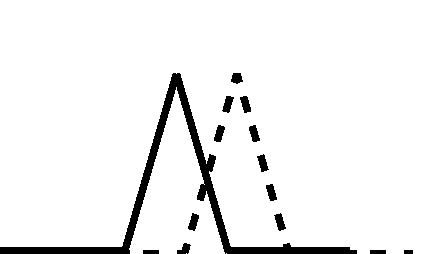
\includegraphics[width=\textwidth]{./figures/invariants/hposition}
 		\caption{Temporal Position}
 	\end{subfigure}
 	~
 	\begin{subfigure}{.45\columnwidth}
 		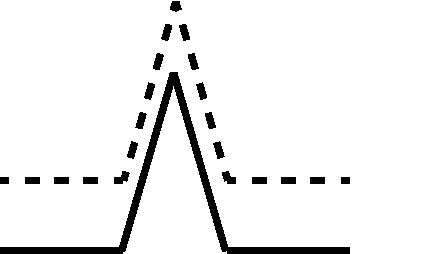
\includegraphics[width=\textwidth]{./figures/invariants/vposition}
 		\caption{Vertical Position}
 	\end{subfigure}
 	~
 	\begin{subfigure}{.45\columnwidth}
 		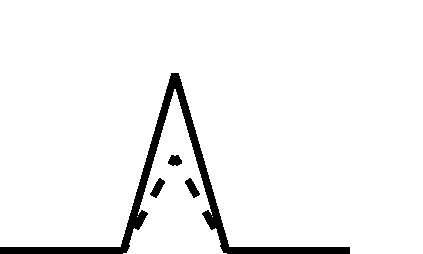
\includegraphics[width=\textwidth]{./figures/invariants/amplitude}
 		\caption{Amplitude}
 	\end{subfigure}
 	~
 	\begin{subfigure}{.45\columnwidth}
 		
\includegraphics[width=\textwidth]{./figures/invariants/size}
 		\caption{Query Size}
 	\end{subfigure}
 	
 	\begin{subfigure}{.45\columnwidth}
 		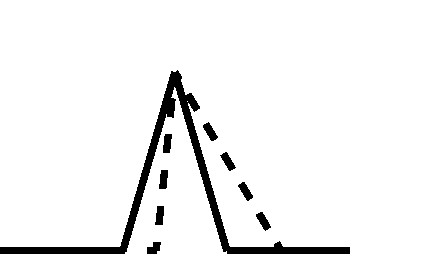
\includegraphics[width=\textwidth]{./figures/invariants/warp}
 		\caption{Time Warp}
 	\end{subfigure}
 	~
 	\begin{subfigure}{.45\columnwidth}
 		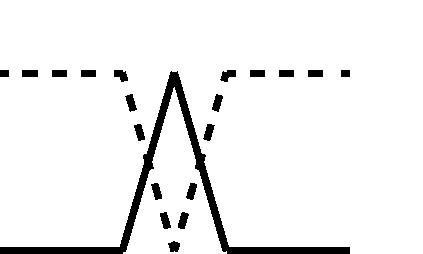
\includegraphics[width=\textwidth]{./figures/invariants/sign}
 		\caption{Sign}
 	\end{subfigure}
 	~
 	\begin{subfigure}{.45\columnwidth}
 		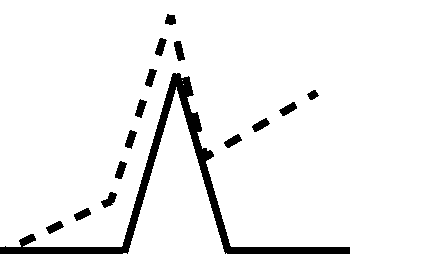
\includegraphics[width=\textwidth]{./figures/invariants/trend}
 		\caption{Trend}
 	\end{subfigure}
 	~
 	\begin{subfigure}{.45\columnwidth}
 		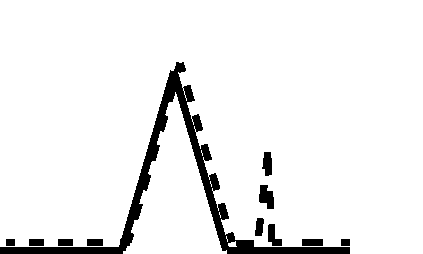
\includegraphics[width=\textwidth]{./figures/invariants/noise}
 		\caption{Noise}
 	\end{subfigure}
 	\caption{A catalog of invariants (or tolerances) for time series matching. For each invariant, assuming a ``spike'' shaped query (the black line), the signal represented by the dotted line would count as a valid match. The analyst's intended meaning of a query might have several implicit or explicit invariants. The analyst might have a different list of what features are or are not relevant during an analysis session. In order to support the analyst, visual query systems ought to flexibly and dynamically support the inclusion or exclusion of these invariants.  }
 	\label{fig:invarlist}
 \end{figure*}	
}

\newcommand{\expFig}{
	\begin{figure*}
		\centering
		\begin{subfigure}[t]{.8\textwidth}
			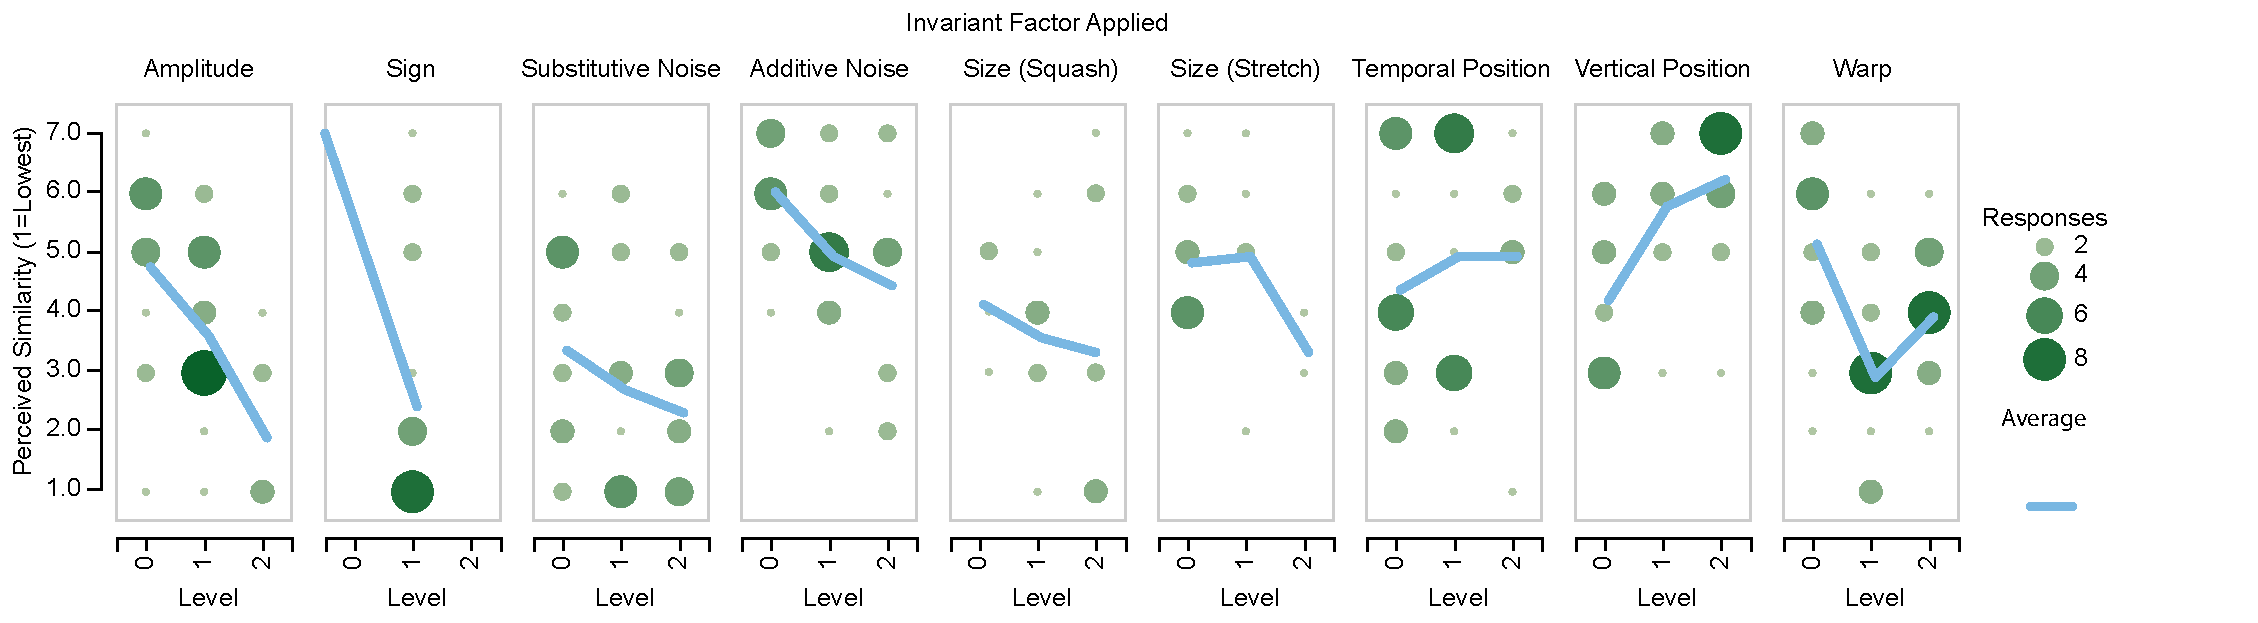
\includegraphics[width=\textwidth]{./figures/exp1-people}
			\caption{Human perceived similarity of area graphs of time series data.}
			\label{fig:exp1people}
		\end{subfigure}
		~
		\begin{subfigure}[t]{.8\textwidth}
			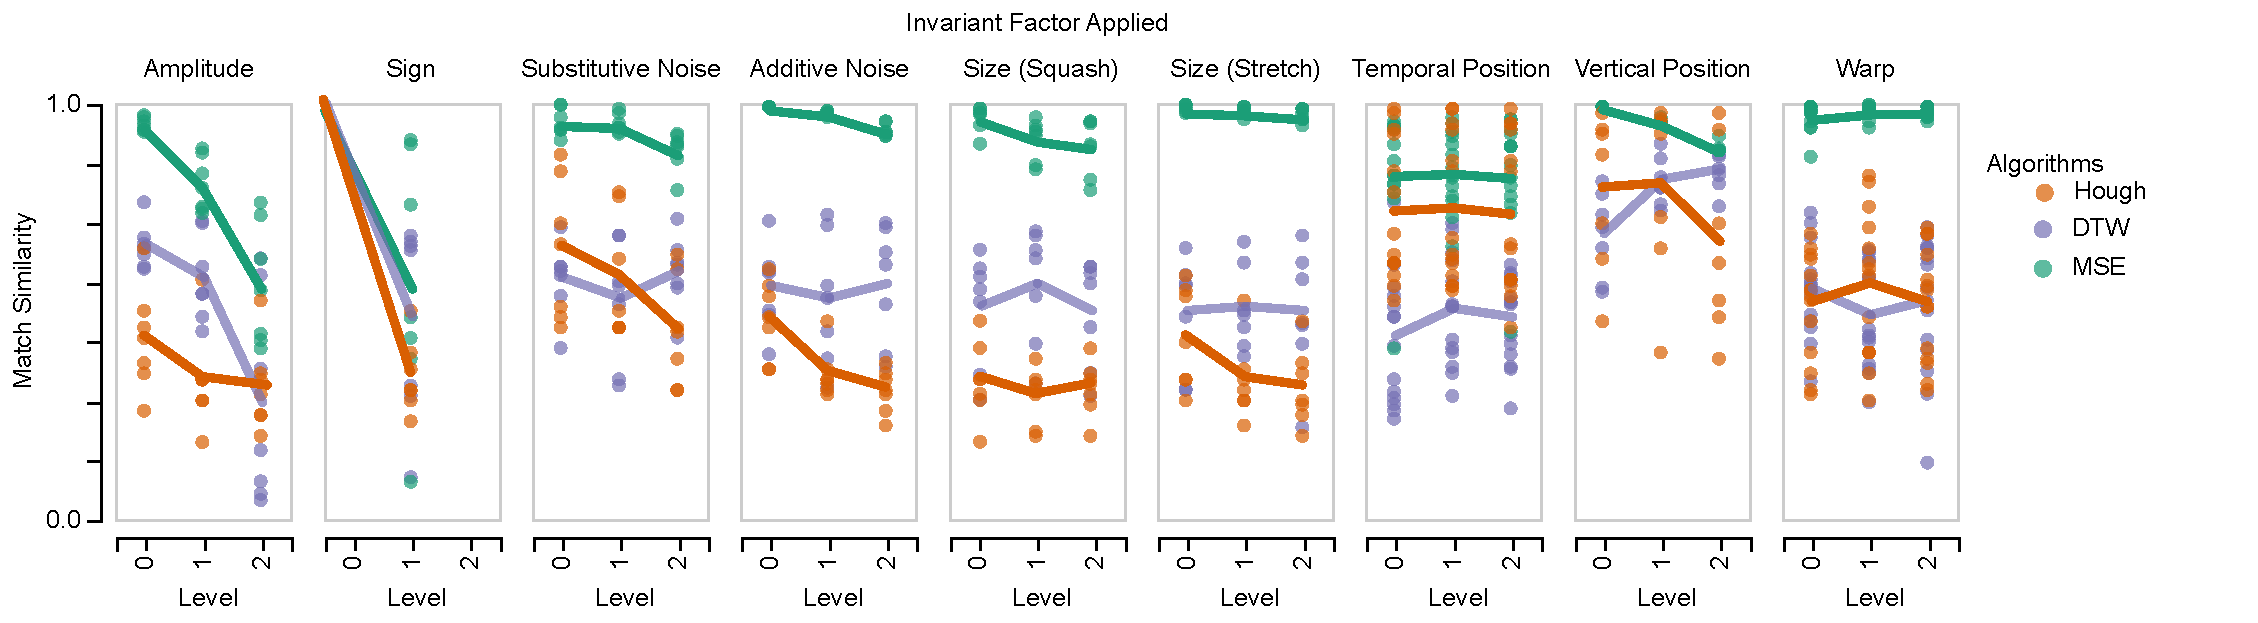
\includegraphics[width=\textwidth]{./figures/exp1-algorithms}
			\caption{Algorithmically calculated similarity. Distances normalized to be in the range $[0,1]$ for each algorithm. }
			\label{fig:exp1algorithms}
		\end{subfigure}
		\caption{Results from our evaluation. Participants were given a target time series, and then had to judge the similarity of the target to a potential match, to which an invariant had been applied. Heterogeneity of human responses show that not all changes to time series result in perceived difference across all viewers. Values are not comparable across conditions, however, slopes are significant: a negative slope represents a sensitivity (similarity falls as the factor increases), while a horizontal line suggests an invariance. This same dataset was then applied to the matching algorithms we present in this paper. Algorithms had varying slopes across the invariants, showing different initial affordances. For instance, additive noise has a significant negative effect on perceived match strength (negative slope). However, only Hough Voting and MSE matching algorithms share a significant negative slope in their match quality as noise is added. Hough Voting and MSE therefore match human judgments of similarity with respect to noise, whereas DTW is invariant to this factor. These data show that algorithmic approaches must be flexible enough to capture the varied mental models of viewers. }
		\label{fig:exp1}
	\end{figure*}
}

\newcommand{\budgetFig}{
	
\begin{figure}
	\centering
	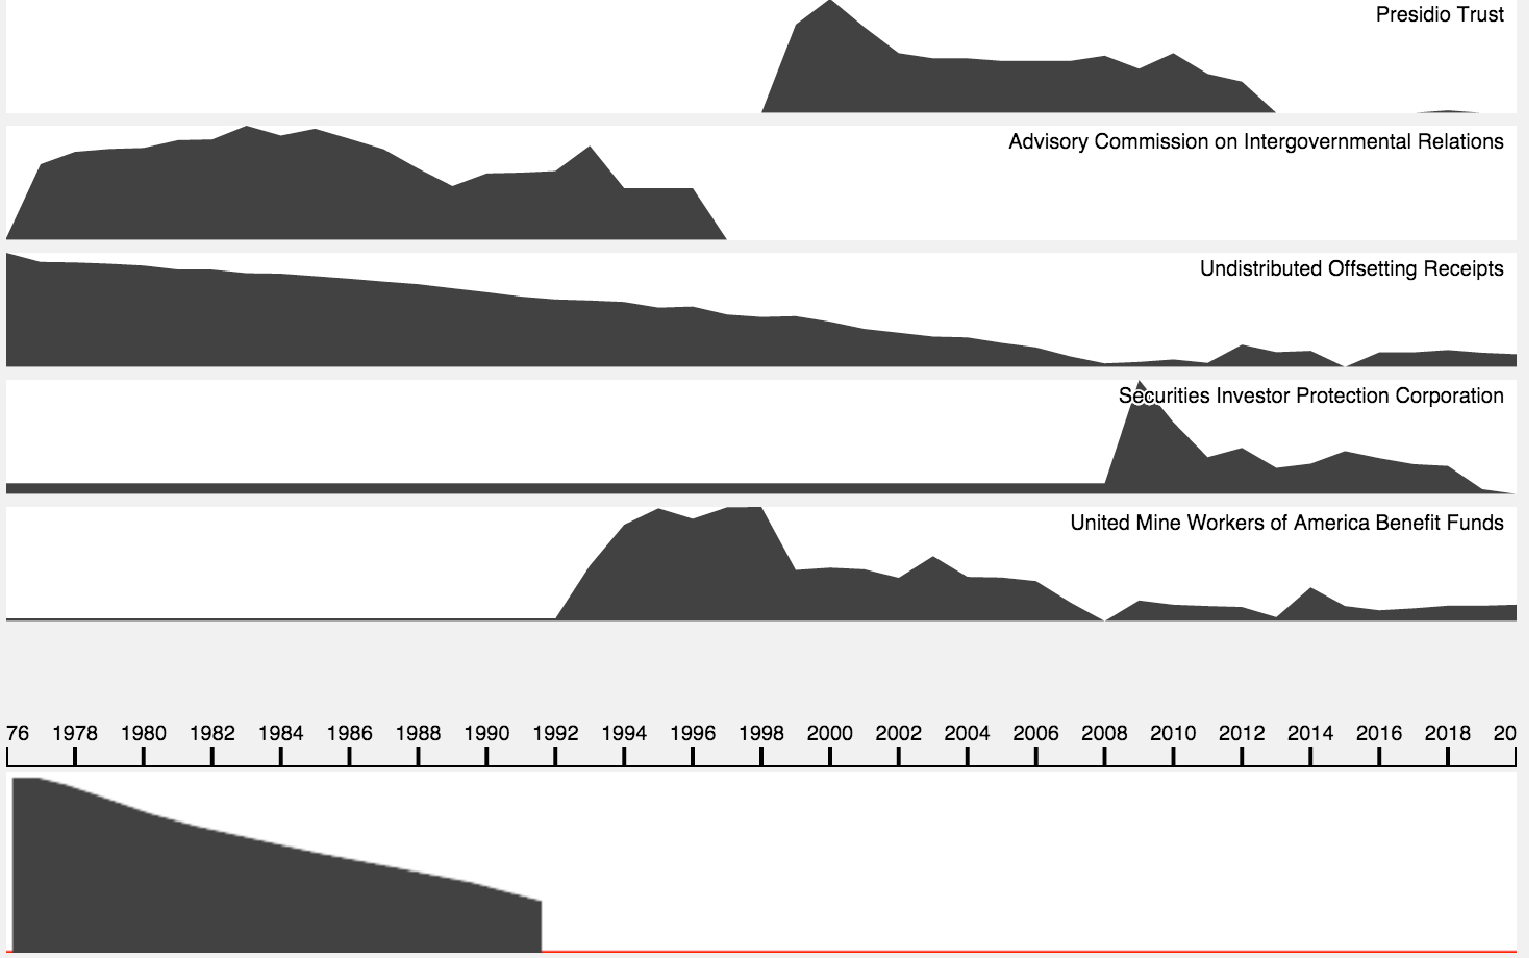
\includegraphics[width=0.7\columnwidth]{./figures/casestudies/budget}
	\caption{A linear query using DTW on the government budget dataset. While some matches have downward slopes, most of the hits have noisy downward trends. We can use these matches to make claims about the presence or absence of patterns in the entire dataset: in this case, agencies tend to lose funding abruptly or noisily, not steadily.}
	\label{fig:budget}
\end{figure}	
}

\newcommand{\eeboFig}{
	
\begin{figure}[h!]
	\centering
	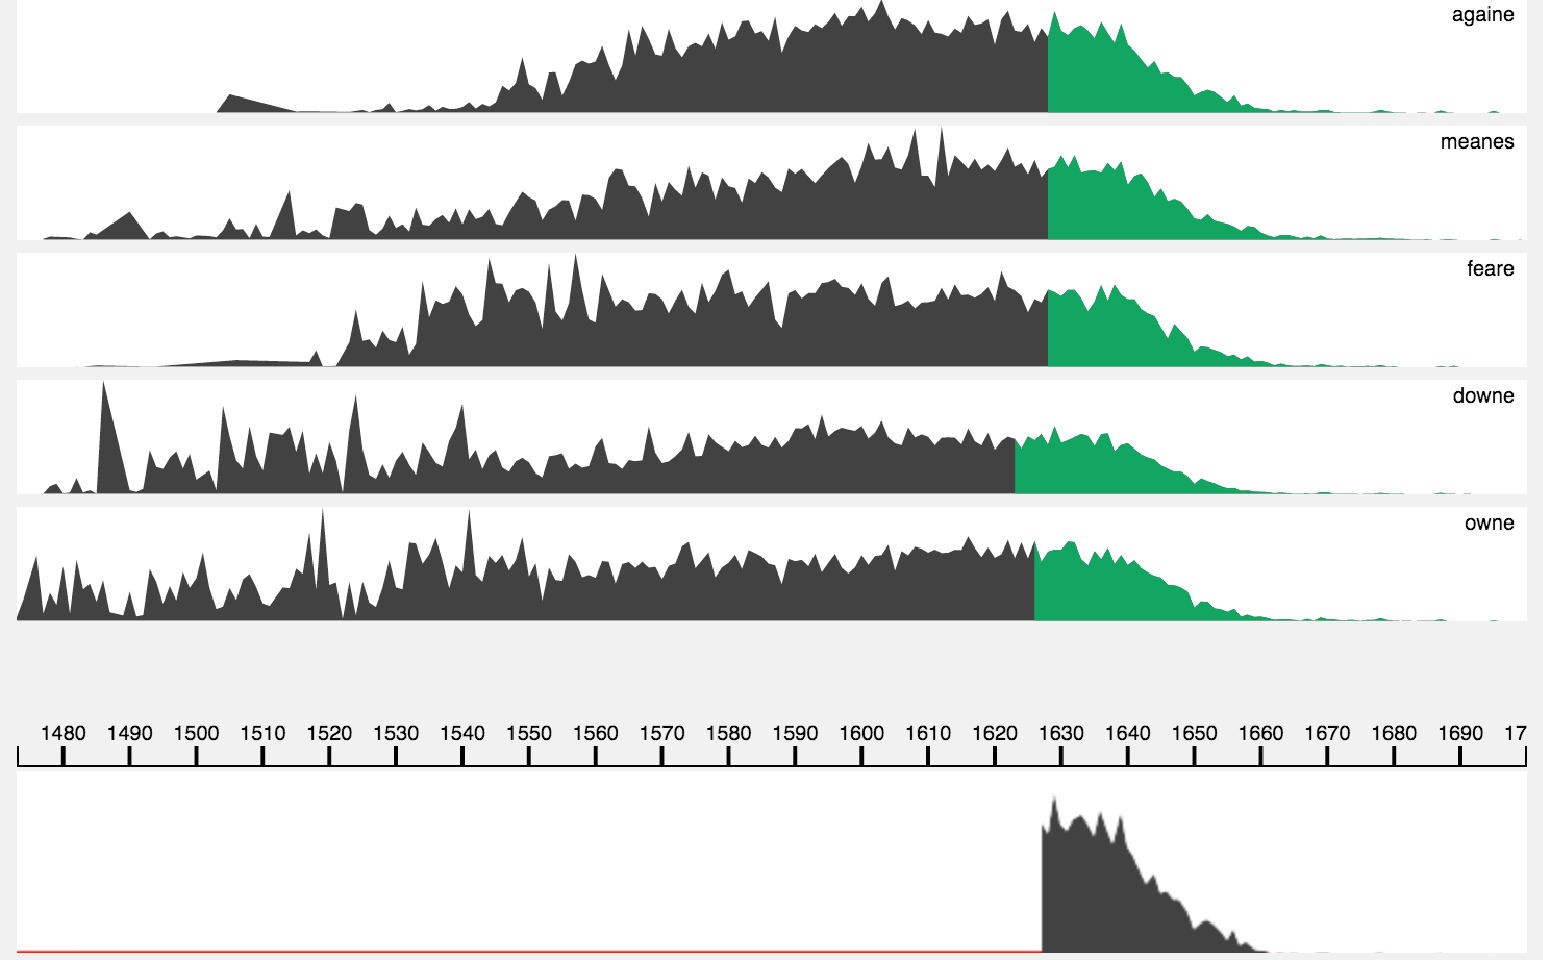
\includegraphics[width=.75\columnwidth]{./figures/casestudies/eebo2.pdf}
	\caption{The top 1000 n-grams from a corpus of 25,000 books printed from 1475-1700 \cite{tcpeebo}. Changes in orthography and print culture over time can create non-standard spellings. In this query, the user has found a decreasing pattern that might indicate a systematic orthographic shift (adding an extraneous `e' to words).}
	\label{fig:eebo}
\end{figure}
}

\newcommand{\stocksFig}{
	
\begin{figure}
	\centering
	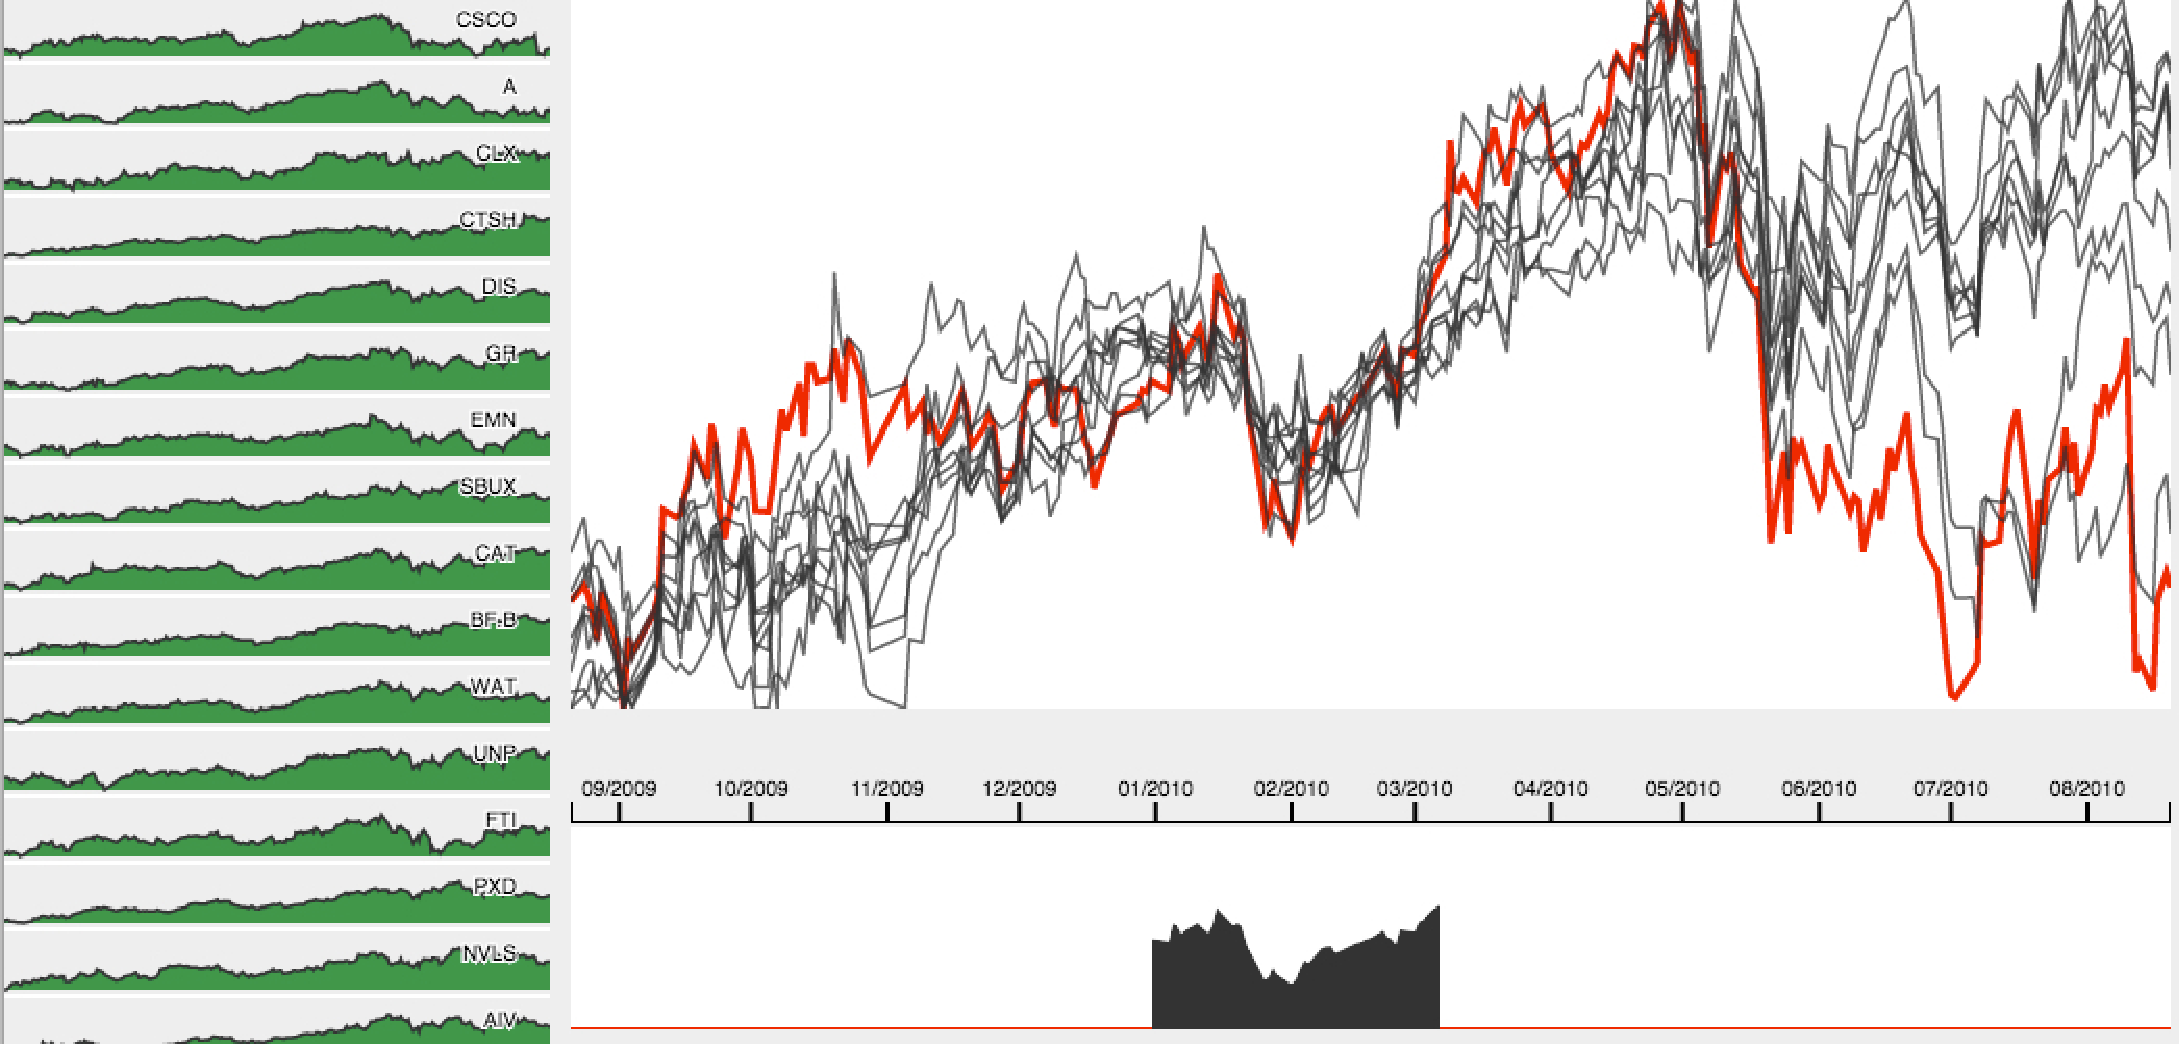
\includegraphics[width=.8\columnwidth]{./figures/casestudies/crash.pdf}
	\caption{Our prototype on a dataset of the daily average price of 524 publicly listed stocks over a one year period from 2009 to 2010. The analyst noticed a characteristic dip at roughly the middle of the timespan that seemed to be common. They selected a series with this pattern, and erased all the irrelevant regions, leaving those areas free to vary. By sorting the results in order of match strength, the analyst is able to look past the top few results and see how common this pattern is in the entire dataset. By juxtaposing the top results on the same chart, the analyst can look for patterns of mutual correlation.}
	\label{fig:stocks}
\end{figure}
}

\newcommand{\houghFig}{

\begin{figure}
	\centering
	\begin{subfigure}[t]{.7\columnwidth}
		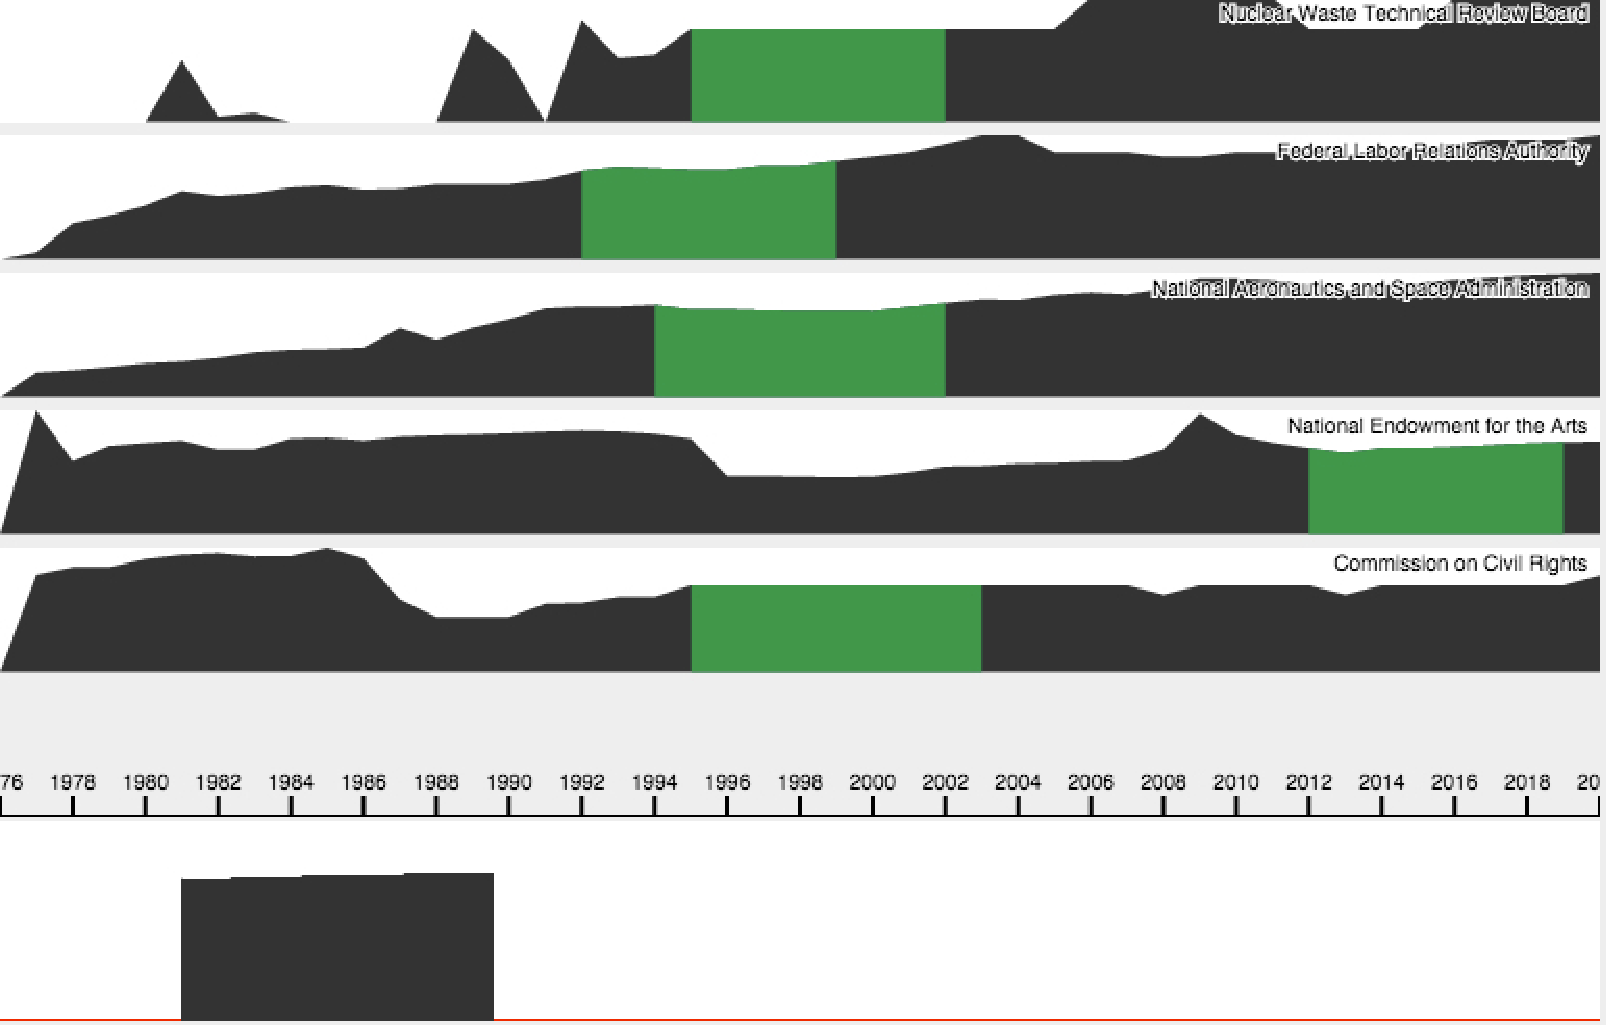
\includegraphics[width=\textwidth]{./figures/msesquare}
		\caption{A box-shaped query using MSE.}
		\label{fig:msesquare}
	\end{subfigure}
	
	\begin{subfigure}[t]{.7\columnwidth}
		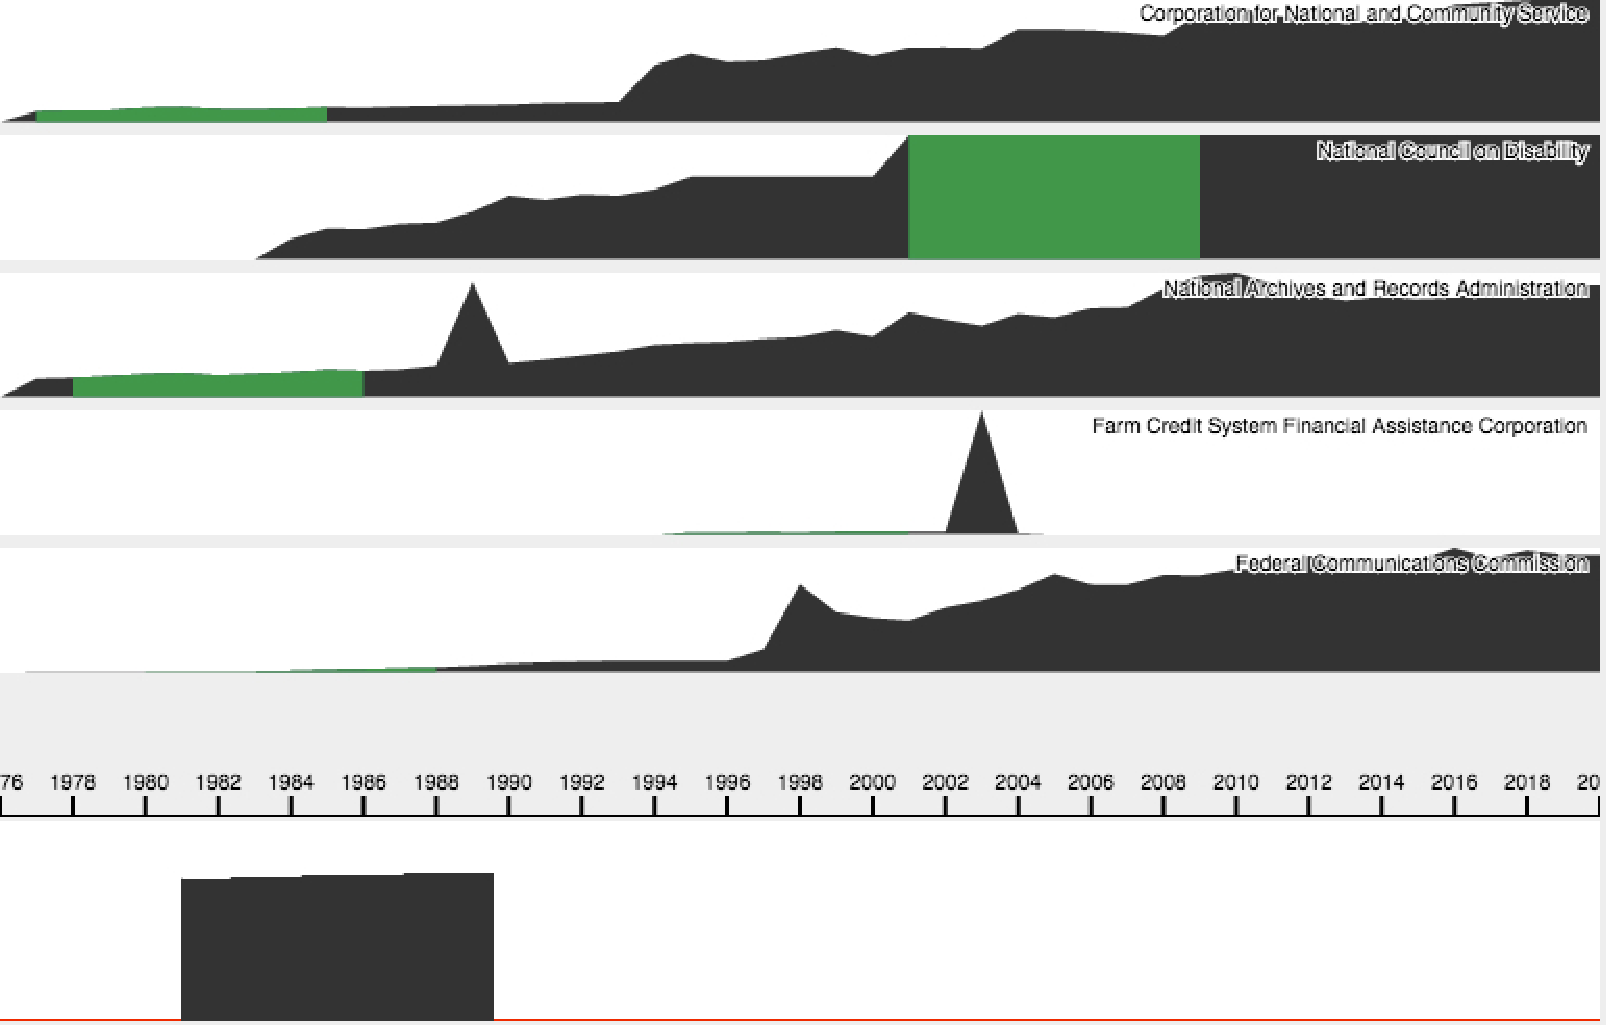
\includegraphics[width=\textwidth]{./figures/houghsquare}
		\caption{A box-shaped query using the Hough Transform.}
		\label{fig:houghsquare}
	\end{subfigure}
	\caption{A box-shaped query on a dataset of the annual budget of 930 U.S. government agencies. MSE will match particular values, finding regions where the budget was, on average, close to the drawn value. Figure \ref{fig:msesquare} shows the results of such a query. Hough voting locates matches that are close in shape to the query, no matter where they occur. Figure \ref{fig:houghsquare} shows these matches, periods of stable budgets.}
	\label{fig:hough}
\end{figure}	
}

\newcommand{\dtwFig}{

\begin{figure}
	\centering
	\begin{subfigure}[t]{.45\columnwidth}
		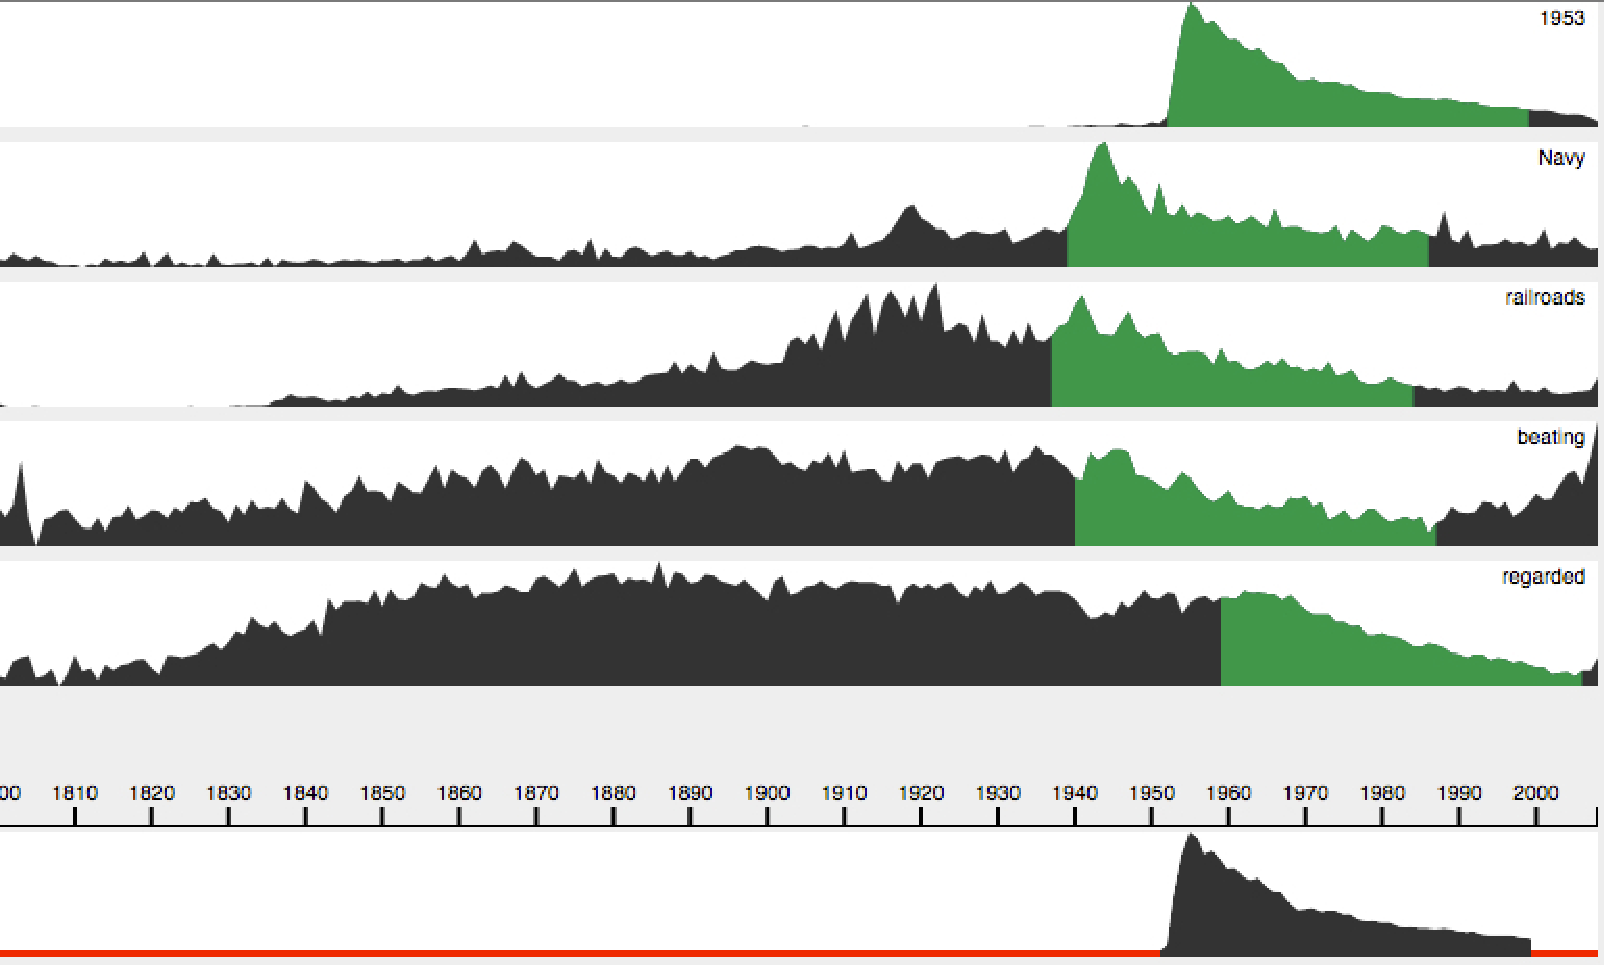
\includegraphics[width=\textwidth]{./figures/mseyear}
		\caption{A query by example using MSE.}
		\label{fig:mseyear}
	\end{subfigure}
	~
	\begin{subfigure}[t]{.45\columnwidth}
		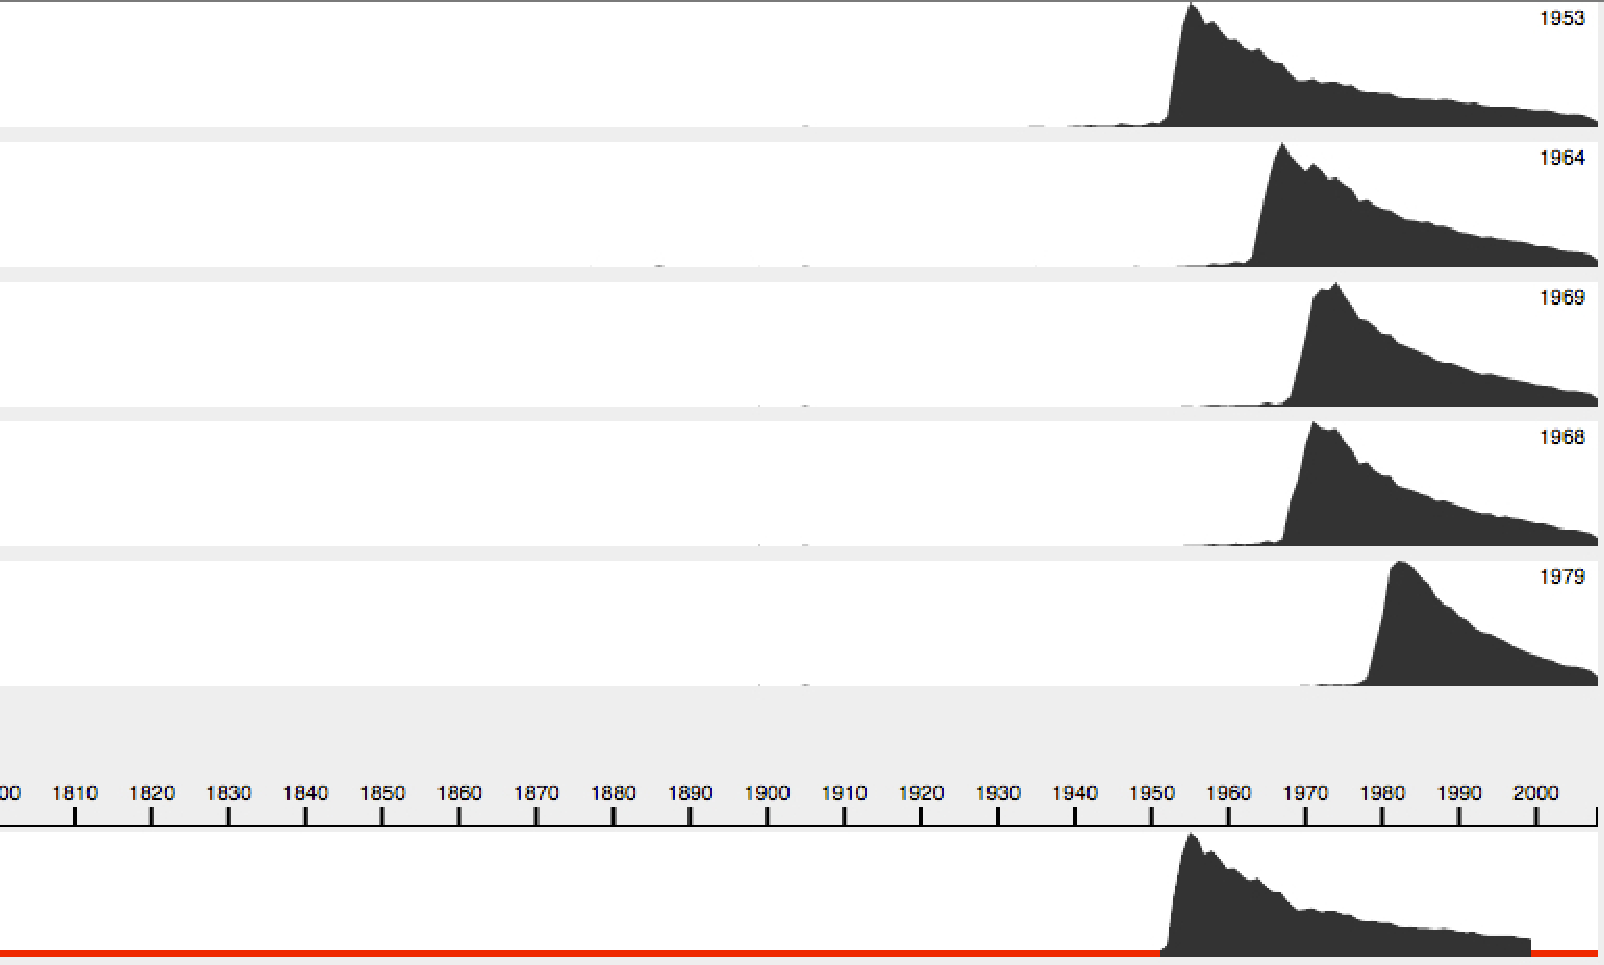
\includegraphics[width=\textwidth]{./figures/dtwyear}
		\caption{A query by example using DTW.}
		\label{fig:dtwyear}
	\end{subfigure}
	\caption{A query-by-example on the top 1000 words in Google n-grams dataset, based on similarity to the word ``1953.'' Initial scholarship has shown that the words for years have a characteristic spike in popularity as they grow nearer, and then a die-off \protect\cite{michel2011quantitative}. The duration of this die-off is of variable length, and appears to be getting shorter and shorter over time (e.g. the die off for ``1953'' was longer than for ``2003''). This change in event timing is distinct enough that the euclidean distance between year words may be quite different. Figure \protect\ref{fig:mseyear} shows the results from the Mean Squared Error (MSE) metric; there are many potentially irrelevant matches. Figure \protect\ref{fig:dtwyear}, by contrast, uses dynamic time warping to align the series. All of top results are year words, allowing comparison across the dataset.}
	\label{fig:dtw}
\end{figure}	
}

\newcommand{\overviewFig}{

\teaser{
	\centering
	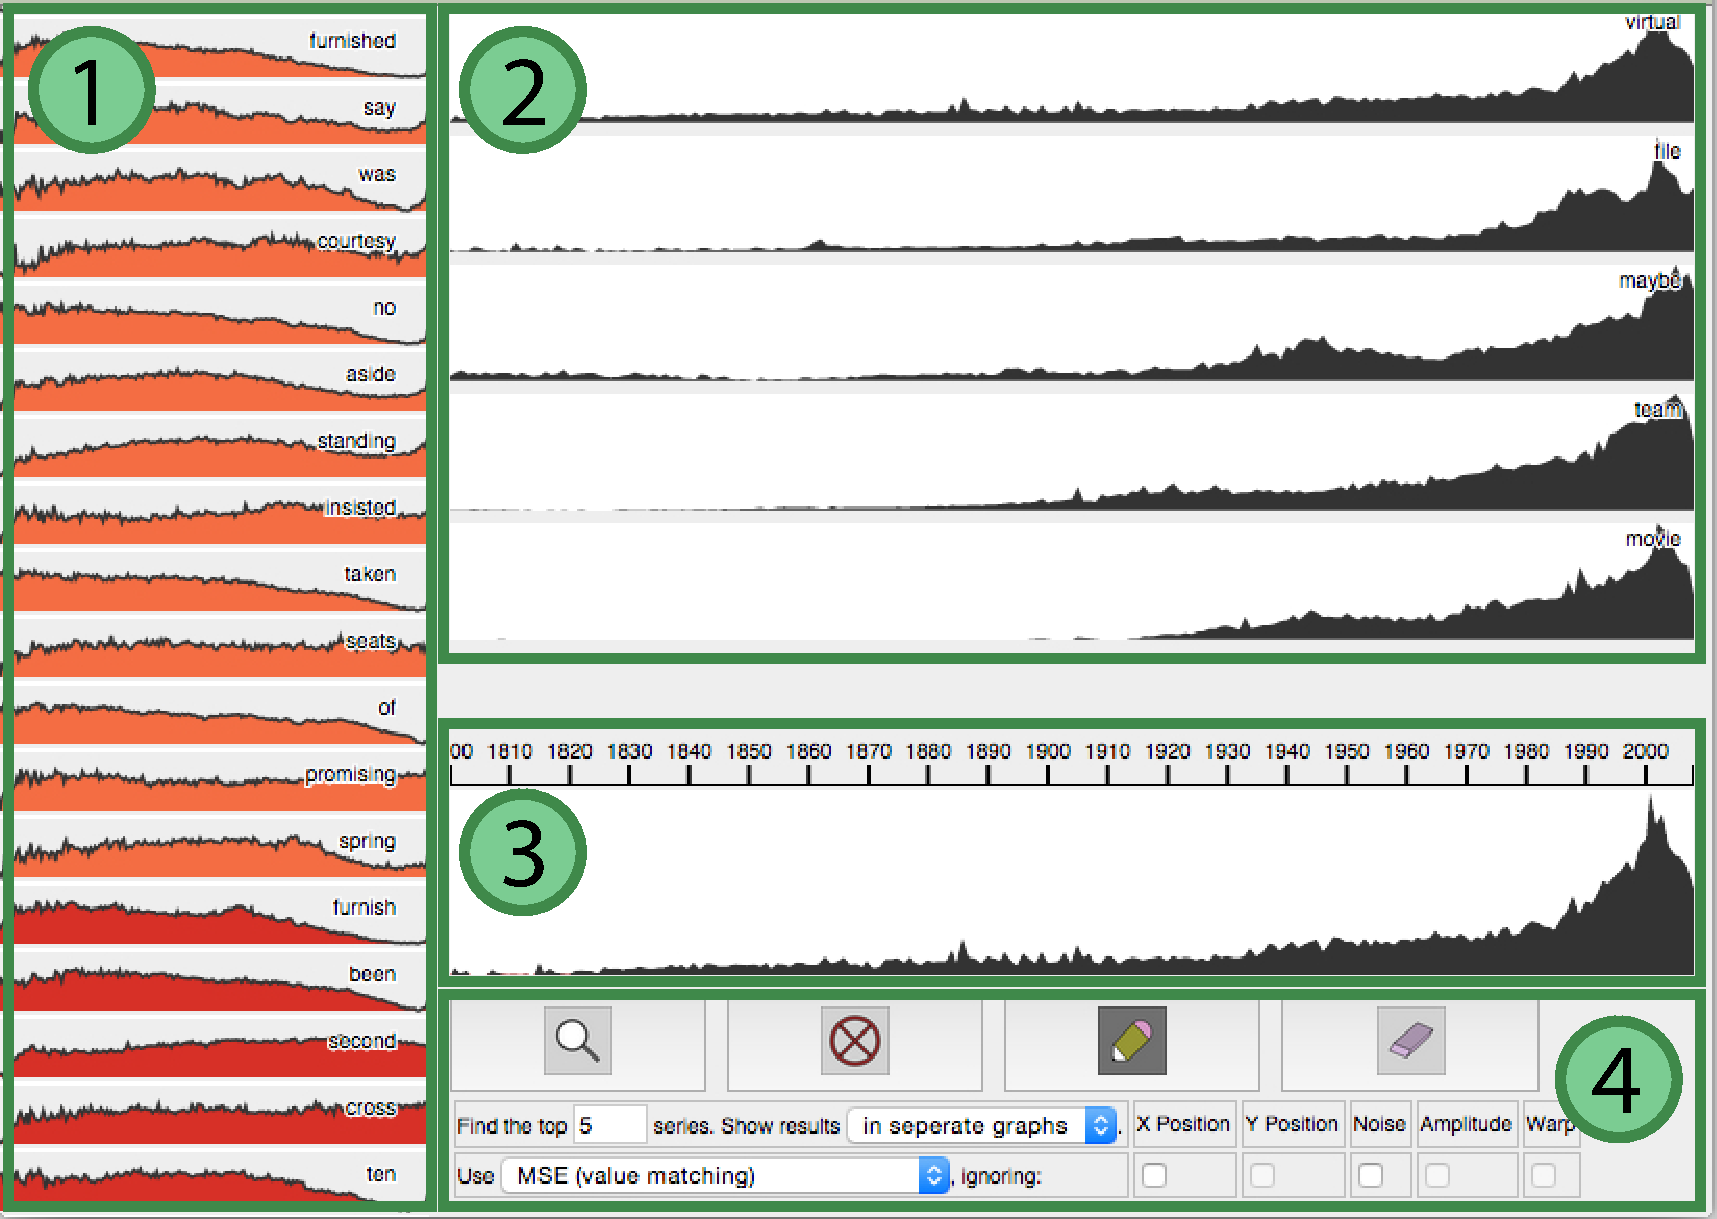
\includegraphics[width=.62\textwidth]{./figures/screenshot2}
	\caption{An overview of the elements of our sketch-based visual query prototype, on the Google N-Grams dataset. Here the analyst wanted to know ``what words have patterns of usage that are most dissimilar to the word `virtual?''' ``Virtual'' is used as a query by example, and the analyst jumps to the bottom of the list of results to find a group of five strong ``anti-matches,'' indicated by their bright red color (including words like ``furnish'' and ``cross''). The components of the system are:
		\\
		\textbf{1}: The scrollable \nameref{sec:smallmultiples} of the entire dataset. Each small multiple is colored according to relative match strength. Here, the analyst has jumped to the bottom of the scroll bar to examine ``anti-matches.''
		\\
		\textbf{2}: The \nameref{sec:results}, showing the top $k$ results for a query. The analyst selects how many results they wish to consider, and whether these results are superimposed in the same plot, or drawn as separate line graphs.
		\\
		\textbf{3}: The \nameref{sec:drawing}. The analyst can sketch their own queries here, or, as in this example, use an existing time series as a base for sketching.
		\\
		\textbf{4}: The \nameref{sec:query} interface and general UI. The large top buttons allow users to execute queries, clear the canvas, draw on the canvas, or erase portions of the canvas, respectively. The lower levels control how results are displayed and what invariants are active.}
	\label{fig:overview}
	}
}

\newcommand{\overviewFigStar}{
	
	\begin{figure*}
		\centering
		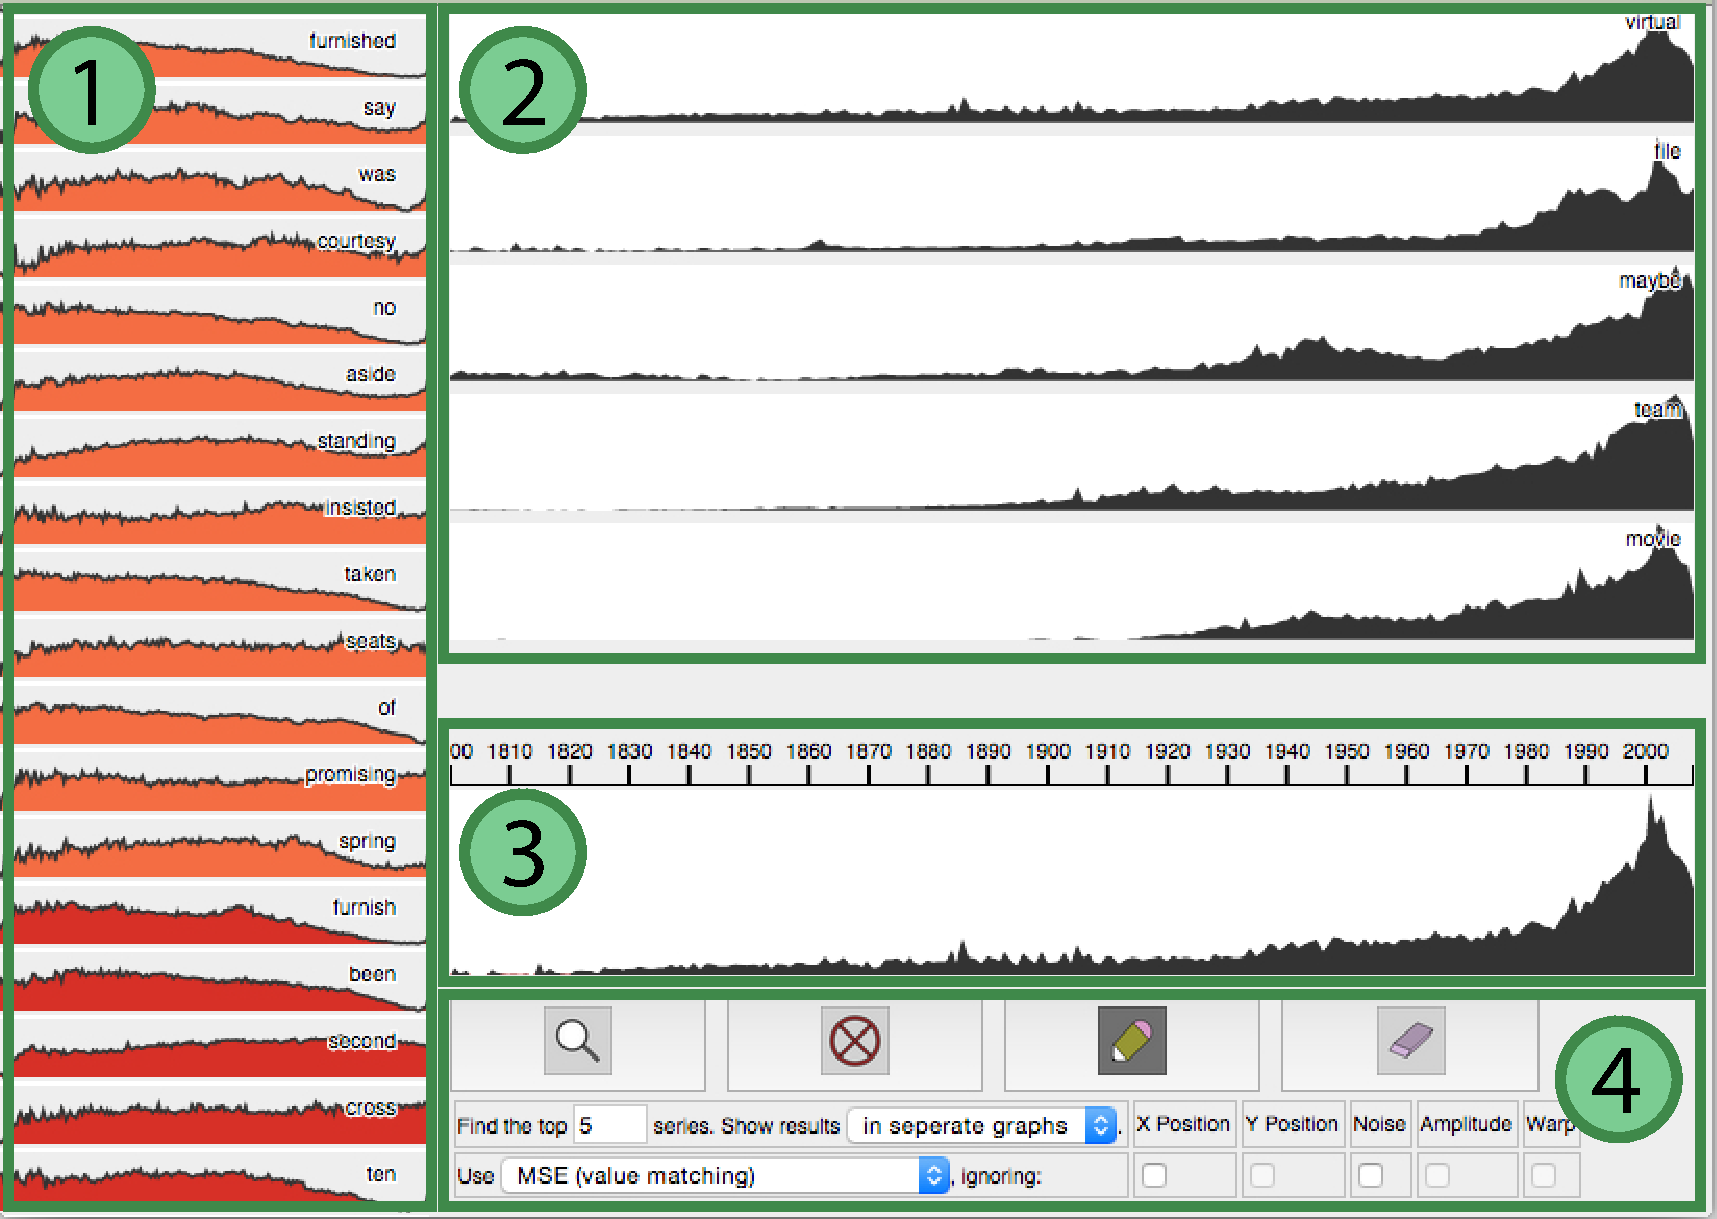
\includegraphics[width=.62\textwidth]{./figures/screenshot2}
		\caption{An overview of the elements of our sketch-based visual query prototype, on the Google N-Grams dataset. Here the analyst wanted to know ``what words have patterns of usage that are most dissimilar to the word `virtual?''' ``Virtual'' is used as a query by example, and the analyst jumps to the bottom of the list of results to find a group of five strong ``anti-matches,'' indicated by their bright red color (including words like ``furnish'' and ``cross''). The components of the system are:
			\\
			\textbf{1}: The scrollable \nameref{sec:smallmultiples} of the entire dataset. Each small multiple is colored according to relative match strength. Here, the analyst has jumped to the bottom of the scroll bar to examine ``anti-matches.''
			\\
			\textbf{2}: The \nameref{sec:results}, showing the top $k$ results for a query. The analyst selects how many results they wish to consider, and whether these results are superimposed in the same plot, or drawn as separate line graphs.
			\\
			\textbf{3}: The \nameref{sec:drawing}. The analyst can sketch their own queries here, or, as in this example, use an existing time series as a base for sketching.
			\\
			\textbf{4}: The \nameref{sec:query} interface and general UI. The large top buttons allow users to execute queries, clear the canvas, draw on the canvas, or erase portions of the canvas, respectively. The lower levels control how results are displayed and what invariants are active.}
		\label{fig:overview}
	\end{figure*}
}

\newcommand{\invariancesFig}{

\begin{figure*}
	\centering
	\begin{subfigure}[t]{.25\textwidth}
		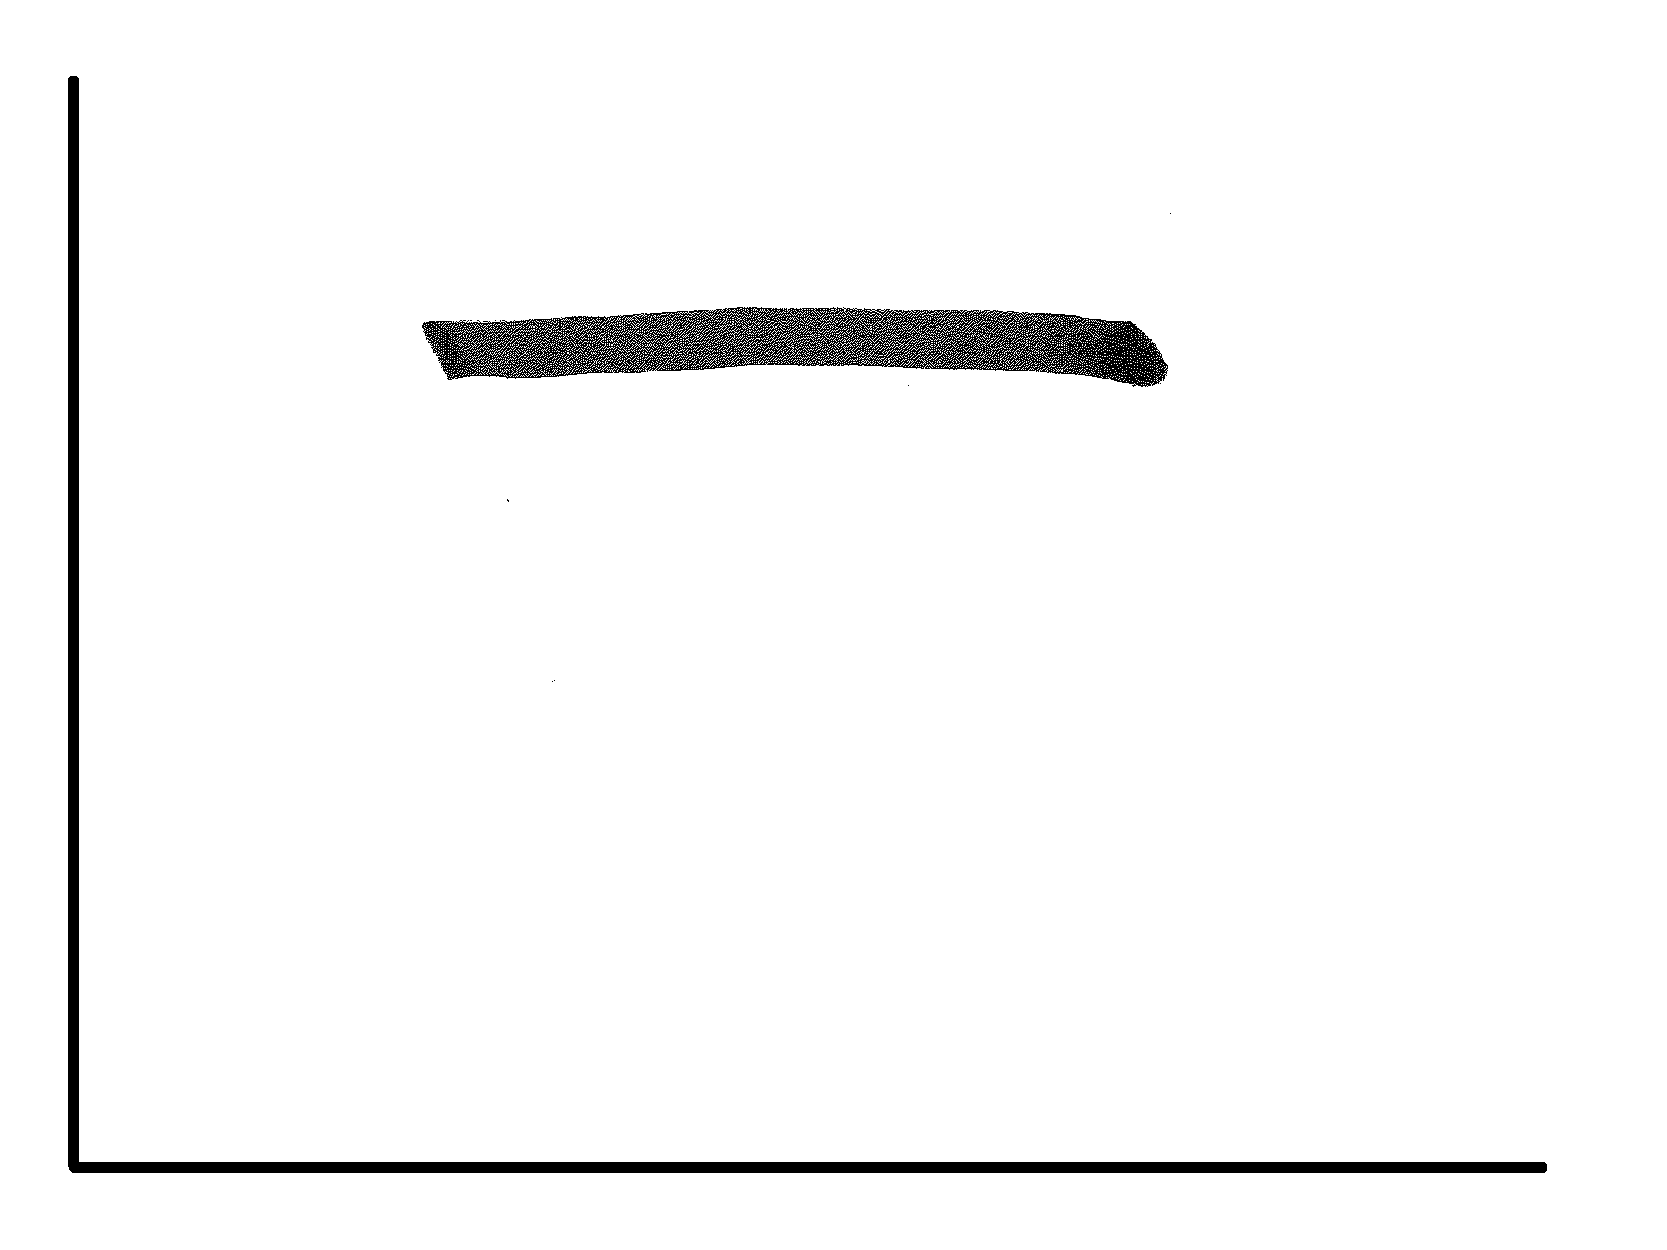
\includegraphics[width=\textwidth]{./figures/sketch2}
		\caption{An input sketch. What counts as a match to this input?}
		\label{fig:sketch}
	\end{subfigure}
	~
	\begin{subfigure}[t]{.25\textwidth}
		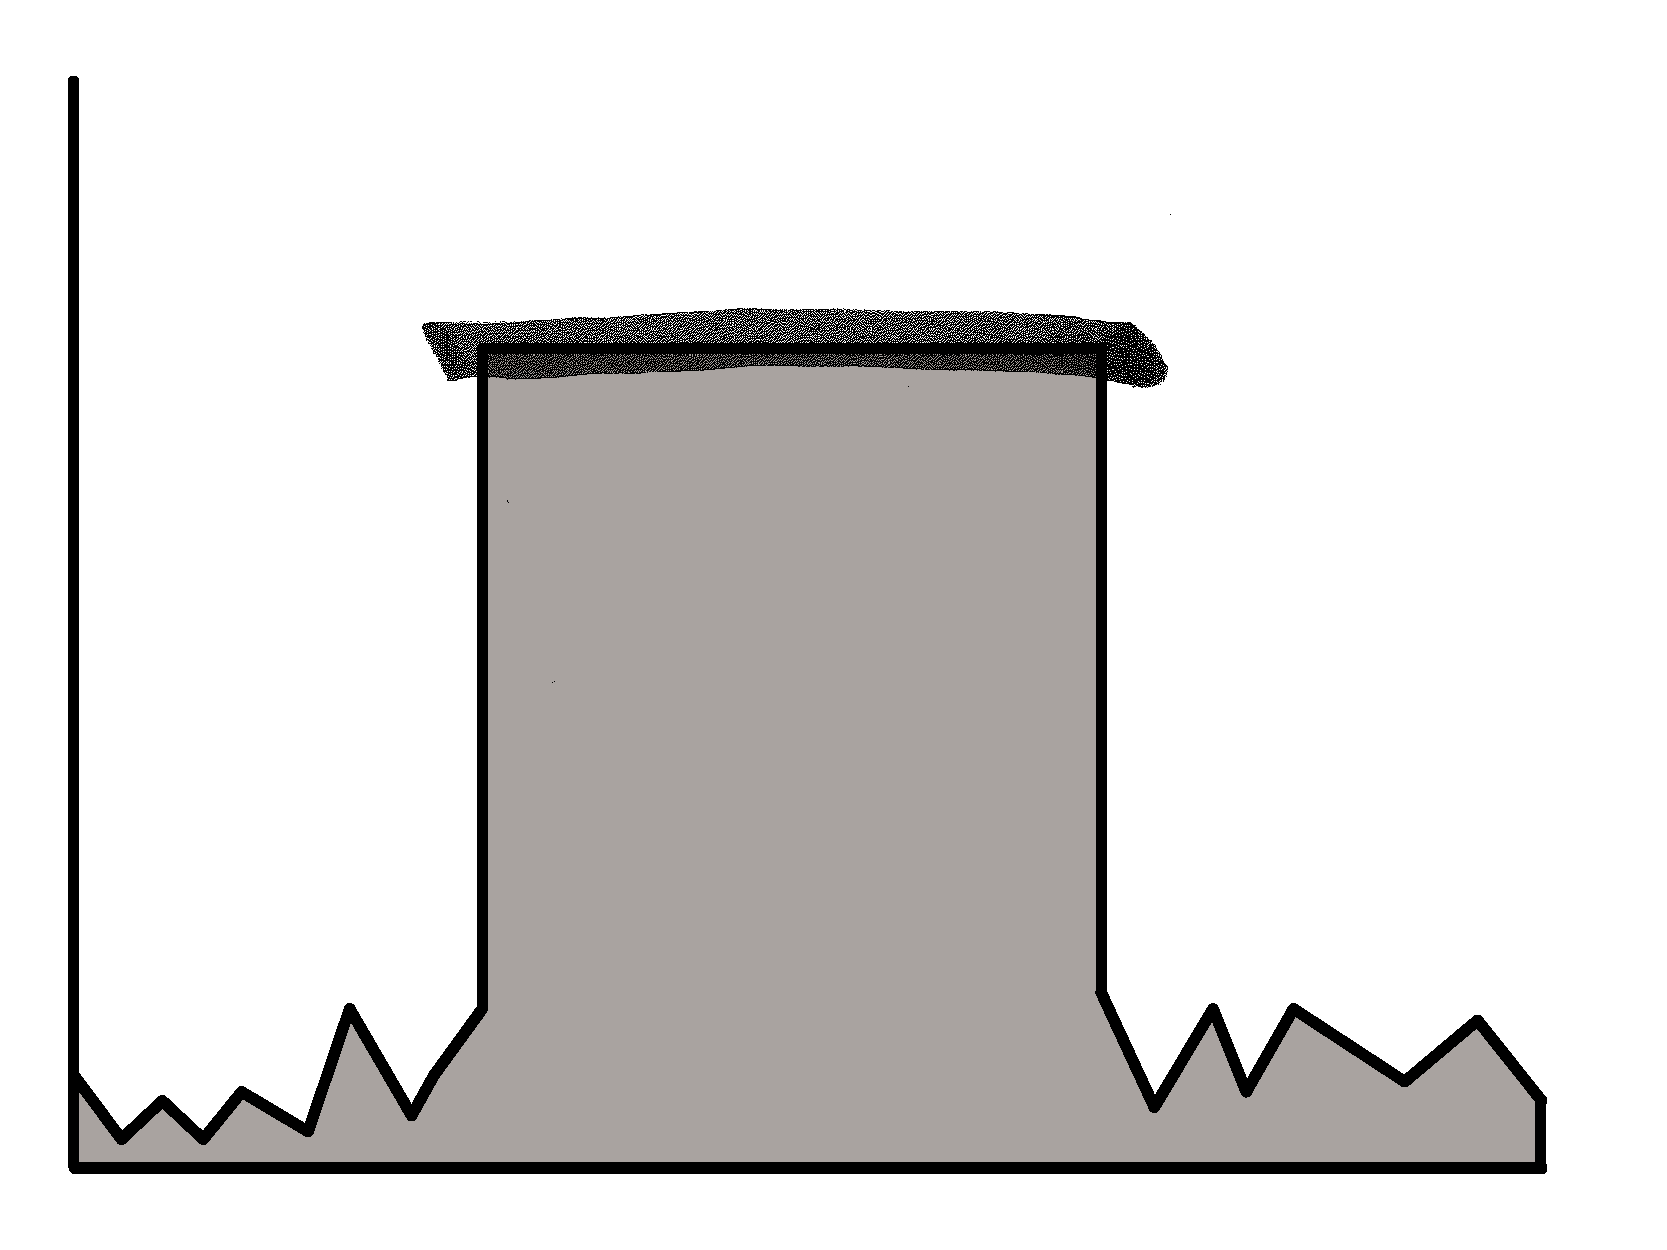
\includegraphics[width=\textwidth]{./figures/exact}
		\caption{A match where, if there is no sketch information, the query is interpreted as being zero.}
		\label{fig:zeroval}
	\end{subfigure}
	~
	\begin{subfigure}[t]{.25\textwidth}
		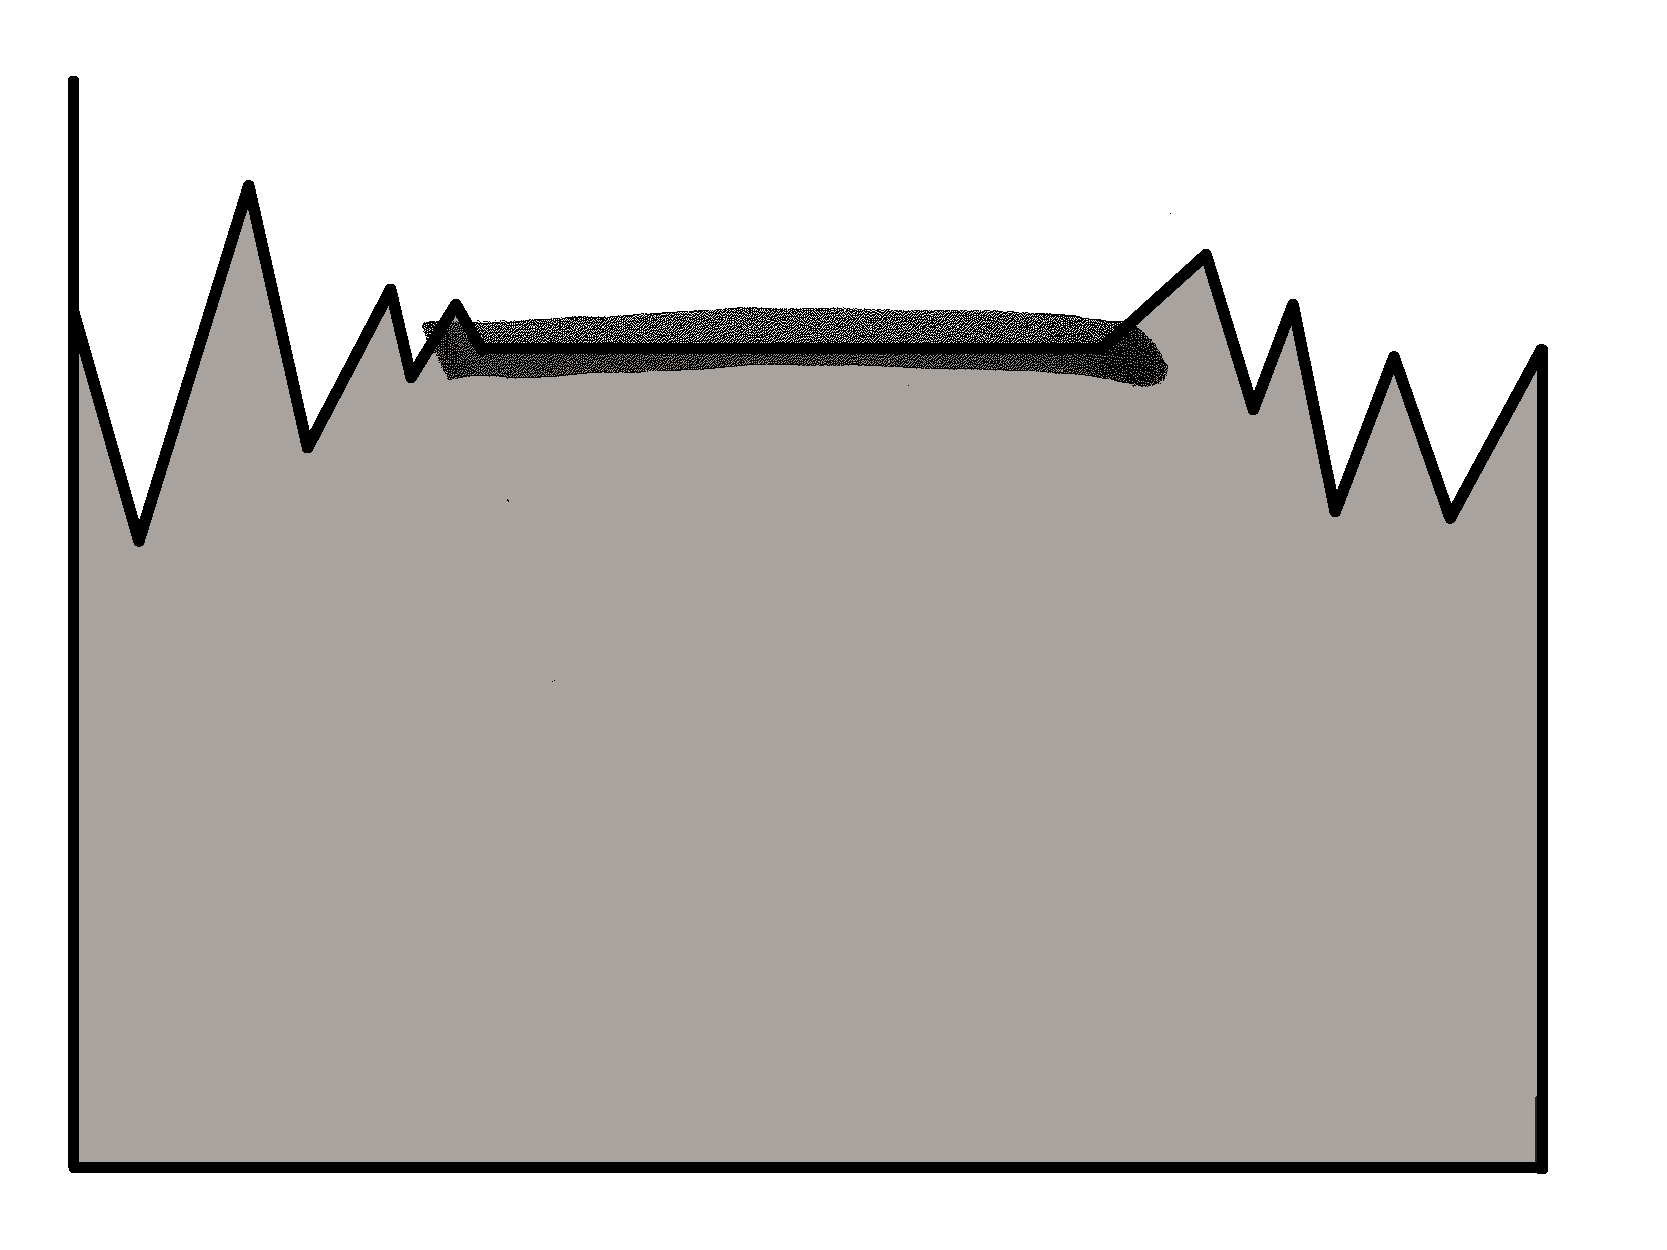
\includegraphics[width=\textwidth]{./figures/dontcare}
		\caption{A match where, if there is no sketch information, arbitrary values will match the query. }
		\label{fig:dontcare}
	\end{subfigure}
	
	
	\begin{subfigure}[t]{.25\textwidth}
		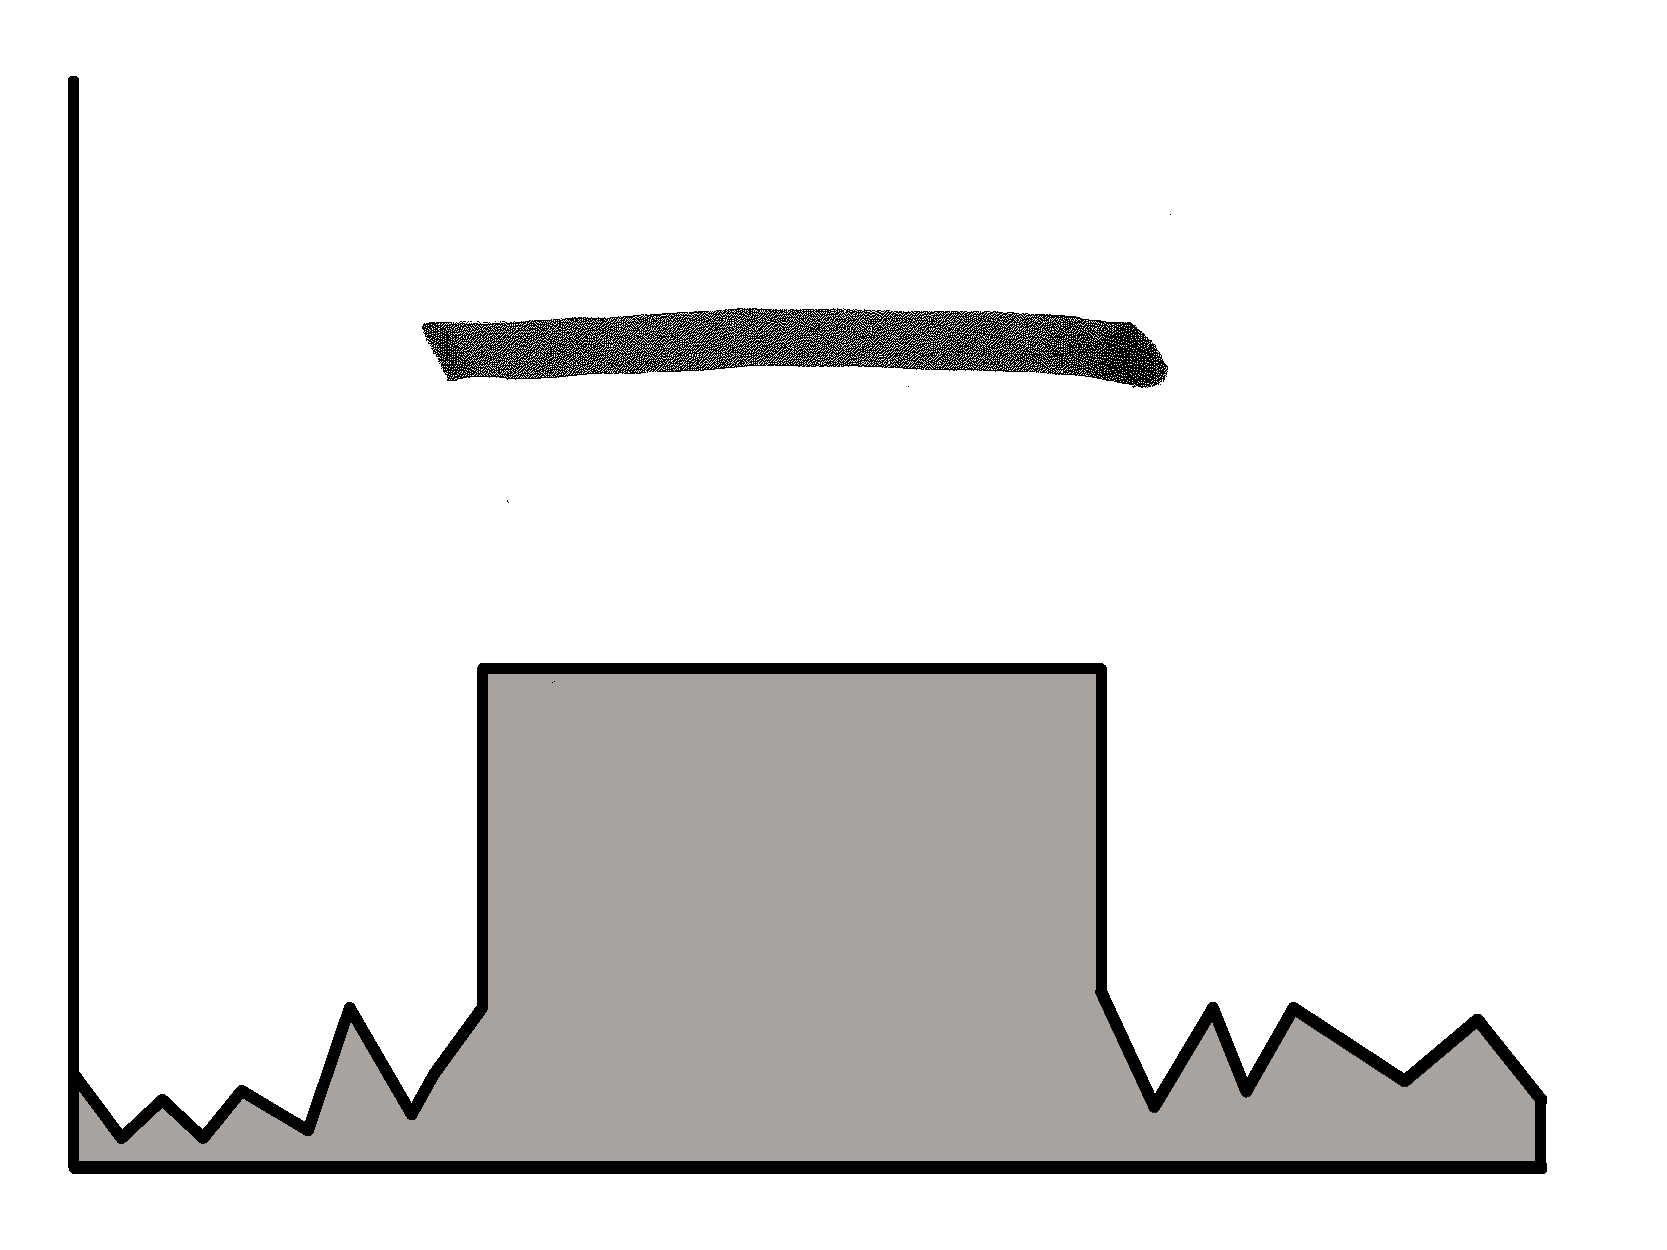
\includegraphics[width=\textwidth]{./figures/amplitude}
		\caption{A match in visual \emph{shape}, but not in \emph{value}.}
		\label{fig:pattern}
	\end{subfigure}
	~
	\begin{subfigure}[t]{.25\textwidth}
		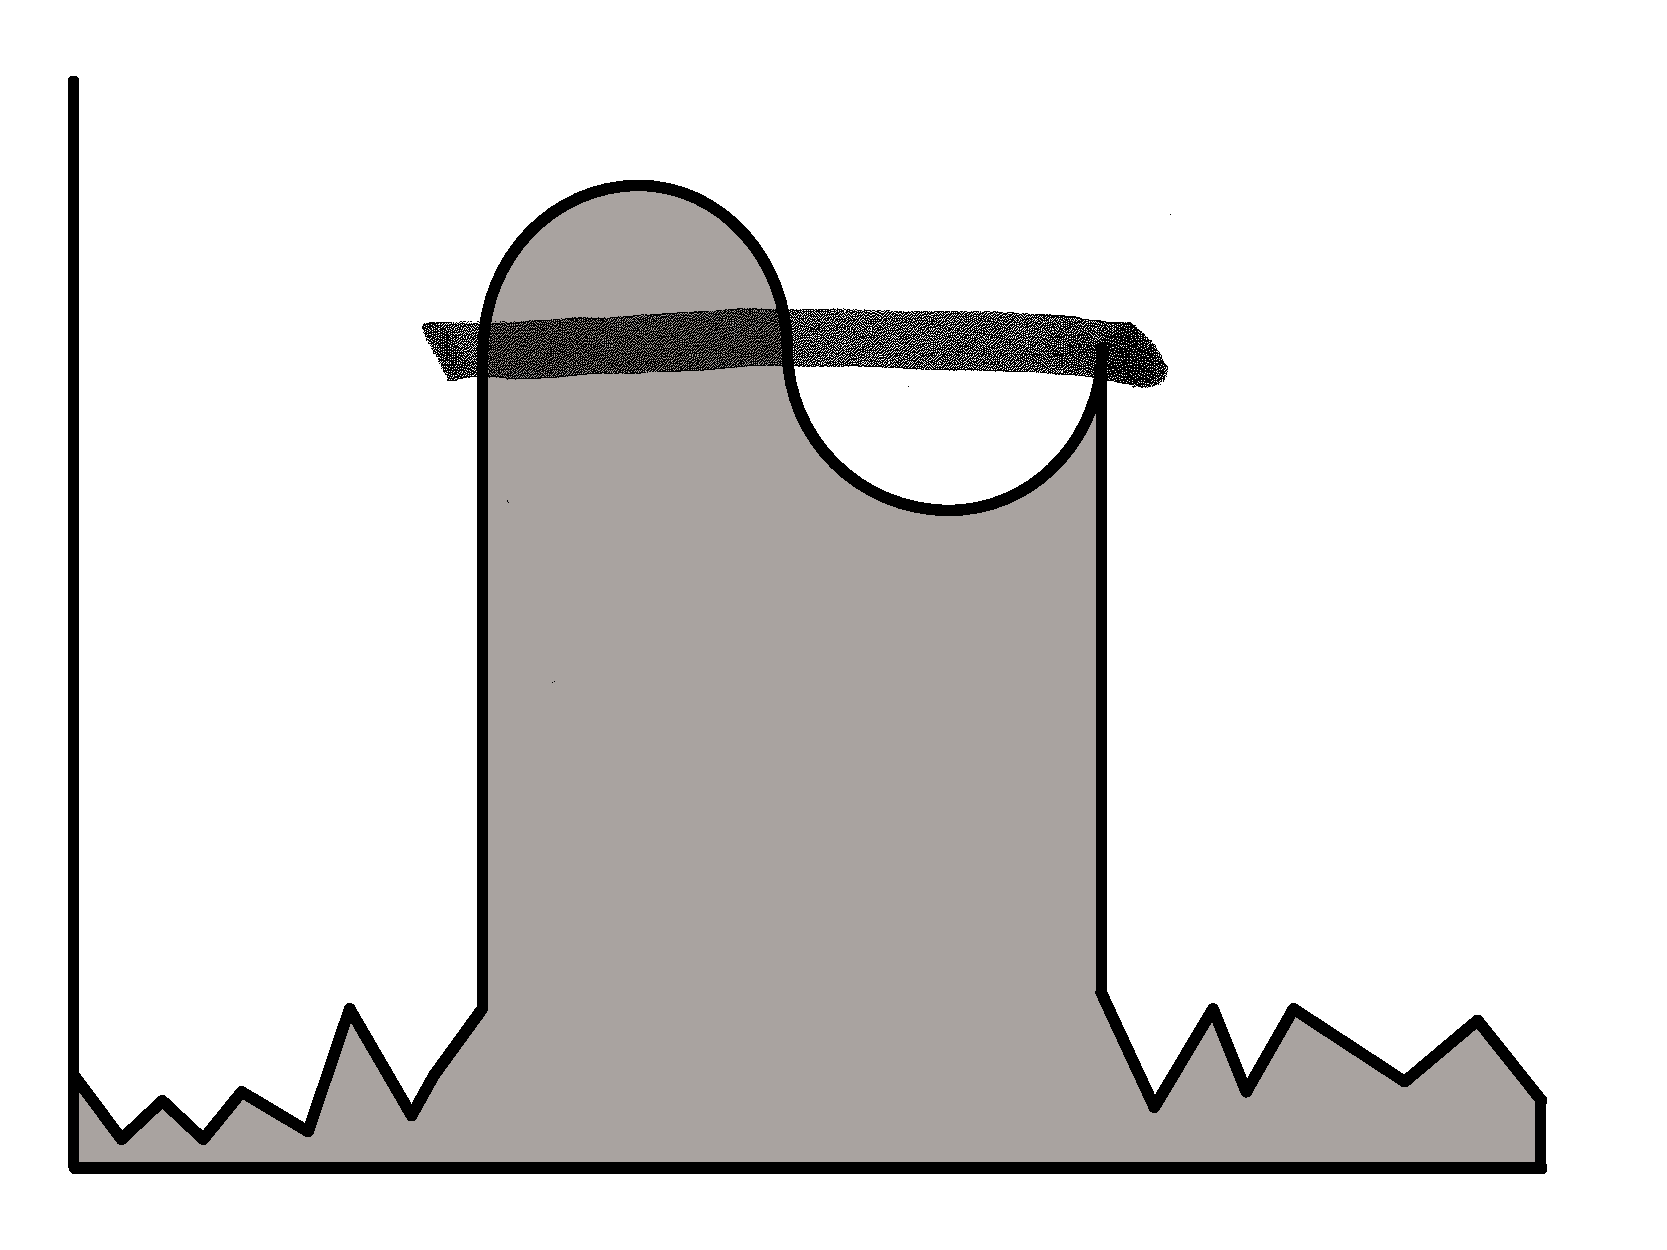
\includegraphics[width=\textwidth]{./figures/average}
		\caption{A match in average \emph{value} but not \emph{shape}.}
		\label{fig:value}
	\end{subfigure}
	~
	\begin{subfigure}[t]{.25\textwidth}
		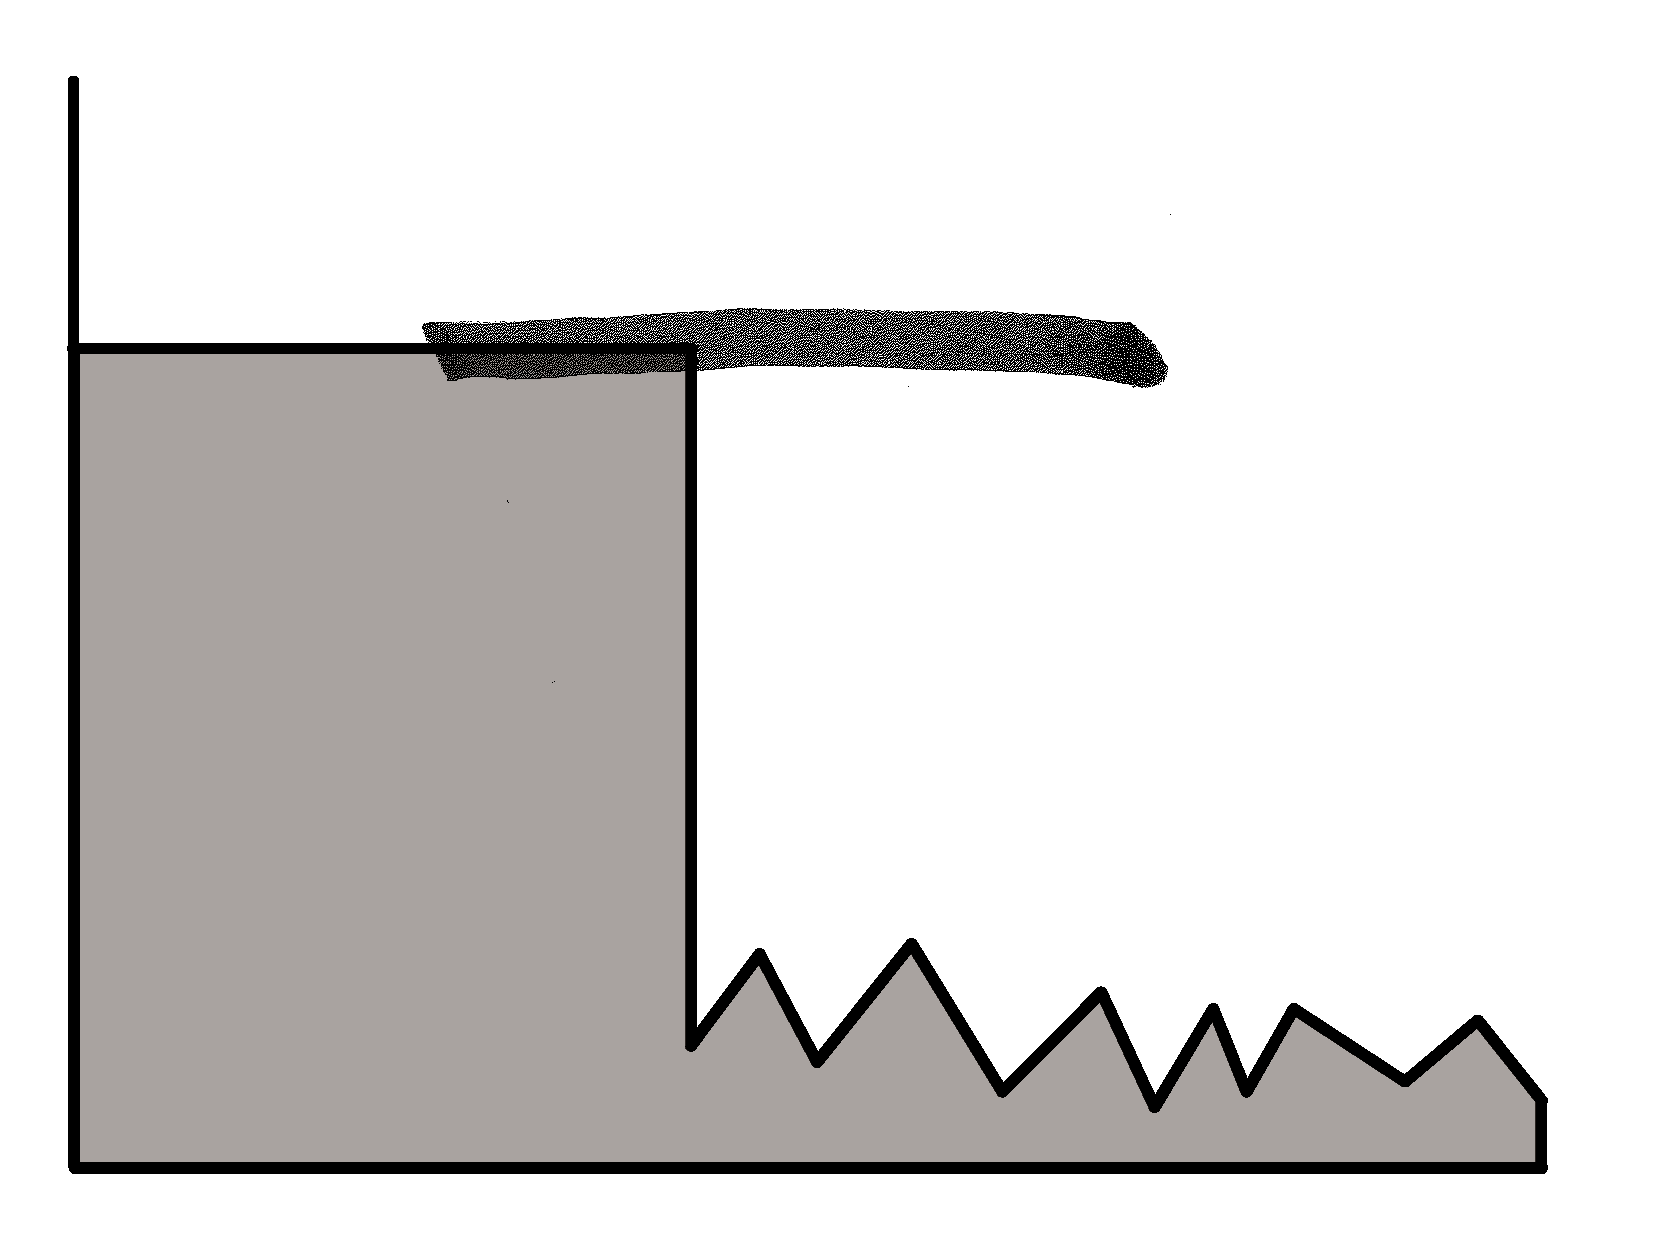
\includegraphics[width=\textwidth]{./figures/temporal}
		\caption{A match that occurs in a different temporal location than in the sketch.}
	\end{subfigure}
	\caption{An example of the ambiguity of sketches as queries. A single sketch can produce many potential matches based on the semantic interpretation of the sketch. Some of these differences can be characterized by one or more invariants (does the analyst care about amplitude, temporal shifts, or noise?), but other differences are fundamental (how should missing values be treated? Should matches be based on the \emph{pattern} of the sketch, or the explicit \emph{values} in the sketch?). These decisions may change over the course of an analysis session. Therefore, visual query systems must provide the option for the analyst to adjust invariants dynamically.}
	\label{fig:invariances}
\end{figure*}
}

\newcommand{\targetFig}{
	
	\begin{figure}
		\centering
		\begin{subfigure}[t]{.45\columnwidth}
			
\includegraphics[width=\textwidth]{./figures/targets/0}
			\caption{Upwards Line}
		\end{subfigure}
		~
		\begin{subfigure}[t]{.45\columnwidth}
			
\includegraphics[width=\textwidth]{./figures/targets/0_a}
			\caption{Amplitude}
		\end{subfigure}
	
		\begin{subfigure}[t]{.45\columnwidth}
			
\includegraphics[width=\textwidth]{./figures/targets/1}
			\caption{Downwards Line}
		\end{subfigure}
		~
		\begin{subfigure}[t]{.45\columnwidth}
			
\includegraphics[width=\textwidth]{./figures/targets/1_i}
			\caption{Sign}
		\end{subfigure}	
		
		\begin{subfigure}[t]{.45\columnwidth}
			
\includegraphics[width=\textwidth]{./figures/targets/2}
			\caption{Sine Wave}
		\end{subfigure}
		~
		\begin{subfigure}[t]{.45\columnwidth}
			
\includegraphics[width=\textwidth]{./figures/targets/2_n}
			\caption{Noise}
		    \label{fig:noisetarget}
		\end{subfigure}	

		\begin{subfigure}[t]{.45\columnwidth}
			
\includegraphics[width=\textwidth]{./figures/targets/3}
			\caption{Tent}
		\end{subfigure}
		~
		\begin{subfigure}[t]{.45\columnwidth}
			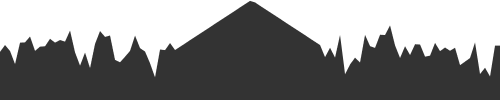
\includegraphics[width=\textwidth]{./figures/targets/3_s}
			\caption{Query Size}
		\end{subfigure}	
			
		\begin{subfigure}[t]{.45\columnwidth}
			
\includegraphics[width=\textwidth]{./figures/targets/4}
			\caption{Perlin Noise v.1}
		\end{subfigure}
		~
		\begin{subfigure}[t]{.45\columnwidth}
			
\includegraphics[width=\textwidth]{./figures/targets/4_t}
			\caption{Temporal Position}
		\end{subfigure}	
		
		\begin{subfigure}[t]{.45\columnwidth}
			
\includegraphics[width=\textwidth]{./figures/targets/5}
			\caption{Perlin Noise v.2}
		\end{subfigure}
		~
		\begin{subfigure}[t]{.45\columnwidth}
			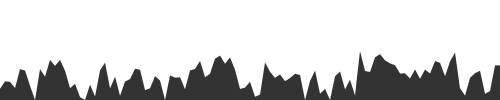
\includegraphics[width=\textwidth]{./figures/targets/5_v}
			\caption{Vertical Position}
		\end{subfigure}	
		
		\begin{subfigure}[t]{.45\columnwidth}
			
\includegraphics[width=\textwidth]{./figures/targets/6}
			\caption{Parabola}
		\end{subfigure}
		~
		\begin{subfigure}[t]{.45\columnwidth}
			
\includegraphics[width=\textwidth]{./figures/targets/6_w}
			\caption{Time Warp}
		\end{subfigure}			
									
		\caption{A full list of the targets from our evaluation, and examples of invariant factors. We generate a pseudo match by applying a factor, and then adding noise to the rest of the series.Two different targets representing pseudo-random noise were used. Additionally, we considered two different characteristics of noise. Substitutive (Fig. \ref{fig:noisetarget}), and additive (not shown).}
		\label{fig:targets}
	\end{figure}
}

%% Uncomment below to include a teaser figure.
\overviewFig
%% Uncomment below to disable the manuscript note
%\renewcommand{\manuscriptnotetxt}{}

%% Copyright space is enabled by default as required by guidelines.
%% It is disabled by the 'review' option or via the following command:
% \nocopyrightspace

%%%%%%%%%%%%%%%%%%%%%%%%%%%%%%%%%%%%%%%%%%%%%%%%%%%%%%%%%%%%%%%%
%%%%%%%%%%%%%%%%%%%%%% START OF THE PAPER %%%%%%%%%%%%%%%%%%%%%%
%%%%%%%%%%%%%%%%%%%%%%%%%%%%%%%%%%%%%%%%%%%%%%%%%%%%%%%%%%%%%%%%%

\begin{document}
%% The ``\maketitle'' command must be the first command after the
%% ``\begin{document}'' command. It prepares and prints the title block.

%% the only exception to this rule is the \firstsection command
\firstsection{Introduction}

\maketitle

%% \section{Introduction} %for journal use above \firstsection{..} instead


\invariancesFig

Analysts working with large numbers of time series cannot examine every time series at once. \emph{Query systems} allow analysts to find subsets of interest in time series data, but they can be complex to learn and require expertise outside of the analysts' domain. In many cases, patterns that are visually easy to describe are difficult to express in a particular query language. \emph{Visual query systems} are an attempt to overcome these issues, allowing the analyst to construct queries visually rather than textually or programmatically. In some cases, these visual query systems will employ the metaphor of \emph{sketching} --- the analyst draws an example of an interesting pattern, and this template is matched against the dataset to highlight subsets of interest, or produce a ranking of potentially interesting time series. However, there are many issues with sketch-based query building, including ambiguity and complexity of input, that have resulted in limited deployment of sketch-based visual query systems for real-world visual analytics problems.

In this paper, we show that consideration of the ambiguity of sketch meaning can enable systems for sketch-based visual querying of time series that support sophisticated analyses without requiring expertise in signal processing or programming languages. A drawback of visual query systems has been a lack of flexibility in the construction and matching of queries. Expectations about sketch meaning are too diverse to capture in one algorithm, no matter how complex; different algorithms generate differing models of salience and accuracy~\cite{eichmann2015evaluating}. Our key insight is to create a connection between the \emph{semantic} flexibility in how sketches are drawn and interpreted, and \emph{algorithmic} flexibility in how the system performs matching and ranking. Creating this connection requires a thorough examination of the potential meanings of sketches. In this work, we introduce the notion of ``invariants'' --- aspects of a time series that the analyst considers irrelevant for finding relevant matches. Key to the notion of invariants is the assumption that a sketch can be ambiguous: the same sketch, when produced under different mental models, can produce different interpretations of good matches. For instance, is a sketch of a straight line (e.g., Fig.~\ref{fig:sketch}) intended to match a period of stability (e.g., Fig.~\ref{fig:dontcare}), or a box shape with sudden rises and falls (Fig.~\ref{fig:zeroval})? 

We built up our understanding of the range of sketch interpretations through a participatory design exercise. We instantiated our ideas about sketch-based querying into a prototype system that runs in the browser.  Our system provides a variety of matching algorithms to support different types of visual queries. We performed a crowd-sourced study examining how invariants affect perception of similarity, and compared these results to the capabilities of our algorithms. 

The contributions of this paper are three-fold. 1) Drawn from a participatory design exercise, we present a vocabulary of invariants: properties of a time series that are free to vary without affecting perceived match strength. 2) We present the results of a crowd-sourced study showing how these invariants affect subjective matches on synthetic data. 3) Lastly, we present a prototype query system (Fig.~\ref{fig:overview}) that supports many invariants through the use of a suite of flexible matching algorithms. This prototype has been applied to many real-world datasets, and embedded with analysts in different domains. 

\section{Related Work}

Sketching is a powerful and expressive mode of interaction. Lee et al.~\cite{lee2012beyond} highlight the benefits of interaction techniques beyond mouse, menu, and keyboard. Sketch-based and pen and touch interaction techniques afford naturalistic and detailed expressive power without extensive training or domain knowledge. Sketch-based systems have been used to locate images of interest in image and video datasets~\cite{flickner1995query,kato1992sketch}, to prototype UI elements~\cite{landay2001sketching}, and to create impromptu visualizations~\cite{lee2013sketchstory}. Using sketches for query generation has proven difficult, given that specifying temporal queries is nuanced and often under-defined~\cite{monroe2012exploring}.

In the following sections, we discuss visual query systems: systems that use visual components to drive the formation of queries. We treat sketch-based visual query systems as a separate case. Our system seeks to combine advantages from general visual query systems, such as their flexibility and depth, with sketched-based systems, which are naturalistic and easily transferred across domains.

\subsection{Visual Query Systems}

Hochheiser \& Shneiderman~\cite{hochheiser2004dynamic} developed an early visual query system for time series data, which relied on the central interaction method of the ``time box'' --- the analyst draws a rectangular region spanning a range of both time and value. The dataset is then filtered by removing series that do not enter the box. By creating and linking multiple boxes, analysts can query for complicated temporal patterns. Later extensions would afford some ``fuzziness'' in the boundaries of the time box~\cite{keogh2002augmented}.

The Querylines system~\cite{ryall2005querylines} takes a similar filter-based approach to visual querying. Instead of boxes, the analyst specifies line segments that act as constraints: for instance, the analyst could filter out all queries that have a value below a given line. The analyst may also specify whether these line segments represent hard or soft constraints. This non-binary approach to filtering, and providing feedback that indicates whether an analyst has created an over-constrained query, is integral to designing robust sketch-based query systems that afford complex query specification.

Another technique for constructing visual queries is to develop a vocabulary of motifs, and then build queries using these basic shapes as components~\cite{gregory2012shape}. For instance, the system can create detectors for basic shapes like sinks or spikes, and then use these detected shapes as landmarks for analysis, or allow the analyst to concatenate shapes into a sophisticated feature-based query. This technique also allows the abstraction of time series into a simpler discrete set of events~\cite{lan2013temporal}.

Relevant to our work is an extension of the timebox interface by Buono et al., where the analyst selects a particular time series, draws a timebox around a region of interest, and this subregion is used as a query by example~\cite{buono2005interactive}. This work recognizes that the analyst requires flexibility and tolerances in how exemplar are used. The system supports this flexibility with four ``transforms'' (binary tolerances): offset, scale, linear trend, and noise. Bak \& Meyer~\cite{bak2011effect} confirm with a user study that, while analysts are capable of composing complicated visual queries to solve problems in large time series datasets, individual analysts will have different strategies for completing the same tasks. In the next full section (\S\ref{sec:invariants}), we discuss the need for \emph{invariants} specifying what properties are or are not allowed to vary during matching, and also recognize the need to support multiple analysis strategies.

Visual query systems can be powerful tools for investigating time series data. These tools enable analysts to describe interesting temporal patterns without having to learn a query language or build up a vocabulary of signal processing terms and features. However, these systems are typically limited in their inputs. Sketching, as free form drawing, allows analysts to come up with queries that the designer of a visual query system may not have anticipated.

\subsection{Sketch-based Query Systems}

Wattenberg~\cite{wattenberg2001sketching} was one of the first to prototype a sketch-based visual query system. In this system, the analyst draws a path and the system calculates similarity to time series in the datasets through simple Euclidian distance. We adapt and expand on this formative work by exploring a larger space of similarity metrics and providing more sophisticated annotation of matches.

TimeSketch~\cite{eichmann2015evaluating} is an emerging sketch-based visual query system. Part of this work involves the use of crowd-sourcing to provide a thorough human-centric evaluation of different similarity metrics for time series. These findings support our decision to employ a variety of different matching systems and parameters, as no one metric was sufficient to consistently generate matches that humans highly ranked --- rather, both algorithm and the particular query were important for determining how humans ranked matches. A difference is that, since our priority was to have low-latency querying in a browser-deployed tool, we employ algorithms not considered by Timesketch. Another difference is that, while TimeSketch presents only the top $k$ results from a $k$-NN search, we use a two-stage visual encoding of results: the top $k$ results as ``large multiples,'' and dynamic sorting of the rest of the data in small multiples. This presentation of results communicates both good matches and the distribution of matches throughout the dataset.

Holz \& Feiner~\cite{holz2009relaxed} recognized that flexibility and tolerance in sketch-based visual query systems do not only apply to calculating matches, but also in using the sketch to specify the query itself. In their work, mouse speed is used to inform the spatio-temporal tolerance of points in the sketched query. We believe that supporting tolerances in both querying and drawing are important components of sketch-based visual querying.

\section{The Semantics of Sketching}
\label{sec:invariants}
For series data, a query system can be thought of as the repeated application of a similarity function comparing an input signal (the query) to a target signal (the potential match), generating a value representing match strength. In most query systems, this similarity function is assumed to be immutable, meaning that the same query will always generate the same set of matches.

For sketching, we cannot assume that two identical sketches have the same meaning, or were meant by the analyst to produce the same matches. Sketches can reflect a variety of cognitive tasks, from visual description to mental model instantiation~\cite{fish1990amplifying}.  \emph{Different mental models can produce identical sketches with vastly different real-world interpretations}. That is, a sketch could be an instance of the analyst trying to replicate a pattern they've seen in the real world, or function as a sort of scratchpad for trying to translate an abstract mental concept into a physical instantiation. Sketches can also be imprecise: drawing introduces noise, and the freeform lines may not perfectly mirror points and values in the dataset. Such ambiguity and imprecision complicate the process of using sketches as \emph{quantitative} input. Fig.~\ref{fig:invariances} shows an example of this ambiguity: the same physical sketch, depending on the assumptions behind it, can produce a wide variety of potential matches.

We use the term ``invariant'' to describe facets of one type of query ambiguity (Batista et al.~\cite{batista2011complexity} use this term similarly). An invariant is a property of either the sketched query or the target that the analyst considers \emph{irrelevant} for determining similarity. E.g., if the analyst draws a pattern at a certain height in the canvas, but considers a valid match to be any series where this pattern occurs, no matter the height in the target series, then their query was invariant to vertical position. Many similarity functions deal with a great number of invariants (see Ding et al.~\cite{ding2008querying} for a survey of such functions, and an analysis of their performance), but this often comes at the expense of complexity and dataset-specific tuning. Nonetheless, providing an appropriate vocabulary of invariants is necessary for designers hoping to capture even a fraction of the full semantic space of sketched input.

\subsection{Participatory Design}
\label{sec:ngrams}

In order to better understand how analysts might use sketches for time series querying, we conducted an initial participatory design exercise with a group of target users. We specifically sought to catalog the kinds of queries potential users wanted to make, the sketches that they wanted to make, and their interpretations of these sketches as queries. This data would lead to a catalog of invariants that a system should support. To conduct the experiment, we constructed a simple sketch-based query prototype that had a drawing canvas for sketching queries and a small multiples display (like the ``Results Pane'' discussed in the final prototype described below). The prototype implemented the simplest matching algorithm (Mean Squared Error (MSE), described later) and showed the 5 nearest matches. We instrumented this prototype in order to collect queries and other usage information, and took notes during the initial deployment.

We presented this prototype to a gathering of the University of Wisconsin Digital Humanities Research Network (DHRN) --- a group of roughly a dozen UW graduate students, professors, and instructional staff in various fields of the digital humanities, including literature, history, library science, and visualization. The members of the group, after consenting to have their queries recorded and being given a brief tutorial, were given unstructured time to explore a time series data set derived from the Google N-Grams dataset with our prototype. The Google N-Grams dataset (available at  \url{https://books.google.com/ngrams}) shows the frequency of words and phrases in the Google Books corpus over time. We selected a subset of this dataset, specifically frequency of the top 1,000 most popular words from 1800 to 2008, as an initial collection of time series for our prototype tool. This resulted in a dataset of 1,000 time series with 209 points per series.

In one hour, the DHRN members made 186 queries. These queries were stored in a database, and hand-analyzed by the paper authors, in conjunction with the notes taken during the session. Most of the queries were of one of two types, partial or exemplar-based queries. 74 of these queries were temporally sensitive partial matches: rather than attempting to find a global match to particular sketched query, the analyst would form queries meant to answer questions of such as ``what words were popular in all eras except the Victorian era?'' or ``What words had the height of their popularity during the Napoleonic War?'' 42 of the queries were exemplar-based --- the analyst would choose a word from the list of small multiples, transfer it to the sketching area, and then attempt to find words similar or dissimilar to the target. In four queries of this type, the analyst modified the transferred query with additional sketching, removing irrelevant sections or inserting new patterns.

We incorporated the feedback we received during this initial session into our final design. It showed the importance of distinguishing zero values from missing values: we had examples of similar sketches that were based on both interpretations of missing regions. For instance, a high value square wave centered on the 1890s was interpreted as both ``what words were most popular in the Victorian era?'' and ``what words were popular \emph{only} in the Victorian era?'' It showed the importance of allowing analysts to create both freeform queries (based purely on sketching) as well as exemplar-based queries (based on existing queries in the dataset). Most significantly, it showed that sketches that were \emph{visually} identical might have different \emph{semantic} interpretations, and that these different interpretations could be characterized by a small set of invariants. 
%181 queries

\subsection{A Catalog of Invariants}
\invarlistFig

By working with the literary scholars, we were able to see a wide range of sketches and discuss their desired interpretations. The interpretations of the sketches could usually be captured by invariants, which fell into a small set that provided a common vocabulary. The fact that different interpretations were desired, sometimes from the same sketch, emphasized the importance of providing user control over what invariants are used by a system in interpreting a sketch.

We present below a vocabulary of invariants for sketch-based queries. Fig.~\ref{fig:invarlist} shows a graphical interpretation of these invariants on a constructed query. It is unlikely that an analyst would wish to have matches where all of these invariants are present simultaneously --- they may have specific constraints in how they wish a query to be interpreted. A query that is invariant to too many factors would potentially match any arbitrary target, and may return many irrelevant results. However, it is likely that the invariants an analyst intends to be active may change over the course of a session. Therefore, similar visual sketches drawn by the same analyst concerning the same dataset may have different intended invariants, and different definitions of what counts as a useful result.

None of these invariants are unknown to the time series analysis community. The term ``invariant'' itself has some precedence (for instance, in Batista et al.~\cite{batista2011complexity}). Our contribution, rather, is to illustrate that 1) these invariants \emph{can} and \emph{do} arise in queries on time series data, even from analysts without statistical or mathematical backgrounds 2) the intended presence or absence of these invariants is \emph{heterogeneous} across users, and 3) query systems should support complex \emph{interactions} between active invariants.

\begin{description}
	\item[Temporal Position] is when the time of the matching portion of the signal is not considered, that is, temporal shifts are allowed.  A prerequisite for partial matching, where we find not just how strongly a query matches a target, but where temporally this match is strongest.
	\item[Vertical Position] allows queries to match independently of their vertical positions. That is, vertical shifts (in value) are allowed.
	\item[Amplitude]  allows queries to match independently of the magnitude of the relative changes within a signal. That is, any scalar multiple of the values are considered the same.
	\item[Query Size] allows for queries to match independently of their temporal scale. That is, uniform scaling of timings are considered the same.
	\item[Sign] allows both the query and its inverse to count as matches.
	\item[Time Warp] generalizes query size invariants to allow for arbitary time warps (that is, stretching some parts and shrinking others).
	\item[Trend] ignores linear trends in the query when considering matches. While this is meaningful in data space, it is especially important for correcting for sketches which may have intended baselines that are not parallel to the bottom of the canvas.
	\item[Noise] allows matches to occur despite the presence of outliers or high frequency values. Of note is that while noise can occur in the dataset, we should also expect some noise in the sketching itself, since many input methods do not afford fluid and accurate drawing.
\end{description}

We also consider two special cases of invariants that are important for selecting matching algorithms. While, in many cases, it is easy to modify existing algorithms to afford the invariants described above and in Fig.~\ref{fig:invarlist}, these particular invariants require fundamentally different strategies:
\begin{description}
	\item[Value] invariance allows matches based on the shape features (the visual pattern) of the query rather than any actual values of the data. For instance, we might want to find all series where there is a gradual rise followed by an abrupt fall: we do not care to what values specifically the series rises or falls, just that those two visual events occur next to each other. Many sophisticated matching algorithms assume that the intent behind a sketch is to create a \emph{pattern} rather than to accurate describe the actual \emph{values} of a query. Algorithms such as the Hough Transform (\S\ref{sec:hough}), Dynamic Time Warping (\S\ref{sec:dtw}), SpADe~\cite{chen2007spade}, CID~\cite{batista2011complexity}, or frequency-space techniques~\cite{chan1999efficient}  will distort or ignore the values of the query in an attempt to capture this pattern.
	\item[Shape] invariance is the opposite of value invariant queries --- we are interested in the numerical values present in the query rather than whatever visual features are present. We do not care about the general shape or pattern of the series, just that it has values close to the ones we specified. E.g., we wish to find a query where the values are consistently above 50. Many simpler similarity functions such as Mean Squared Error (\S\ref{sec:mse}), cosine similarity, and Euclidian distance, are based upon comparison of value.
\end{description}

We present this list to motivate our decision to support multiple matching algorithms and provide groundwork for thinking about how these invariants are often composed in practice. If we have enough algorithmic flexibility to capture a wide space of invariants, we can capture most of the semantic space of sketches without creating too much complexity for either the system to handle or the analyst to navigate. 

Prior work has examined  similar notions of ``elastic''~\cite{ding2008querying} and ``approximate''~\cite{shatkay1996approximate} time series matching, and in general, there exist a wide variety of algorithms that can be made invariant or partially invariant. One potential solution is therefore to attempt to create a single similarity function which is tuned to be appropriately invariant to all of the factors above. We believe that this approach is misguided, because two analysts (or the same analyst at different points in their analysis) might draw a visually similar sketch with very different semantic meanings, expecting very different results based on their internal decisions about invariants. Also, in many cases the analyst does not \emph{want} a particular invariant to be active (for instance, querying for a specific pattern of values at a specific point in time). Therefore, we maintain that the analyst must explicitly inform the query system about particular sets of invariance. Since different algorithms support different sets of invariants, this entails that an invariant-robust visual query system should support multiple similarity measures.

In the following section, we discuss our prototype in detail, with special focus on the matching algorithms we employ, and the invariants they afford.

\subsection{Similarity Measures}

We present three initial algorithms for measuring similarity, sampling general classes of \emph{value-based} (calculates exact differences in value) and \emph{shape-based} (matches general shape or pattern) matching techniques. Mean Squared Error (MSE) is the value-based measure we use. Our shape-based measures are the Hough Transform and Dynamic Time Warping (DTW).

Many algorithms for measuring time series similarity exist, and some have more flexibility in terms of invariance to shifts in amplitude, linear trend, or non-linear warps (see Ding et al.~\cite{ding2008querying} for a survey). However, many of these alternative algorithms are computationally expensive, or have a large parameter space that requires extensive per-dataset tuning. This complexity may be too high in practice, especially given the deleterious effect of latency on visual analytics tasks~\cite{liu2014effects}. Similarly, tuning a particular algorithm to support one set of invariants might come at the expense of support for other invariants; e.g., being robust for noise might involve removal of high frequency values, which can be harmful for shape-detecting algorithms that rely on information in the derivatives. We do not present the following algorithms as an attempt to exhaustively characterize this space. Rather, we present exemplars of algorithm classes that afford different sets of invariants.

\subsubsection{Mean Squared Error}
\label{sec:mse}

The user may wish to query for particular numerical values in a time series. For instance, we may not care about the visual features of the query, but merely the query's numerical similarity to a target. We employ MSE as an exemplar of this class of algorithms.

For two signals S and T, we define the mean squared error as $\sum\limits_{i=1}^{|S|} (S(i) - T(i))^2$. This algorithm is $O( max(|S|,|T|))$ in running time. In practice, on a 4th generation iPad running Google Chrome, this corresponds to query latency of less than 100 ms for our 1000 time series N-Grams dataset (see \S\ref{sec:ngrams} for more information on this dataset). Partial matching requires repeated applications of the MSE algorithm to identify the location with the lowest MSE, raising the complexity to $O( |S| \cdot \frac{|S|}{|T|})$, although low resolution sampling to find local minima and gradual refinement remains linear in complexity with respect to query size. Partial matching, in the worst case (small query, large target), introduces latency on the order of 10 seconds for the N-Grams dataset.

This class of algorithm does not afford many invariants directly. Pre-processing and repeated executions are necessary to reduce the impact of factors such as temporal scale, location, and noise. This preprocessing often introduces tunable parameters that add to both computational and conceptual complexity. For instance, to make MSE invariant to noise, we convolve the target signal with a low pass filter before performing comparison.

\subsubsection{Hough Transform}
\label{sec:hough}

\houghFig

The Hough Transform is an algorithm commonly used for shape detection in computer vision~\cite{ballard1981generalizing,illingworth1988survey}. The core of the algorithm is a voting-based approach that estimates the likely center of a match. Pseudocode of our implementation:

\begin{algorithmic}
	\Require A 2D matrix of initially empty accumulator cells V, a signal S, and a target signal T.
	\For{Point $i$ in $S$}
	\For{Point $j$ in $T$}
	\State h = $(|T|/2) - j$
	\State v = $($range($T$)$/2) - T(j) + S(i)$
	\State $V(h,v)$++
	\EndFor
	\EndFor
	
	\State \Return The x-position of the accumulator cell with the maximum number of votes as the match \emph{location}, and the value of this cell as the match \emph{strength}.
\end{algorithmic}

Hough voting is $O(|T|\cdot|S|)$ in running time.  In practice, this can mean query latency of 20 seconds for long queries on our 1000 N-Grams dataset. While there are extensions that increase the number of parameters beyond simply the number of accumulator cells to store, the initial algorithm requires very little per-dataset tuning.

Hough voting is invariant to both temporal shifts and uniform shifts in value (see Fig.~\ref{fig:hough}). The algorithm is also robust to noise, as even if there are some values that are not exact matches, a partial match will still see many votes accrue in the same location. In the pseudocode above, we assume that the accumulator cells have identical resolution to the signal --- in practice, for reasons of both space and robustness, the accumulator cells are a much lower resolution than the signal, so many distinct vote locations are aliased and accumulate in the same cell. Lowering the resolution of the accumulator cell matrix operates as a control over invariants --- fewer vertical cells corresponds roughly to invariance in amplitude, and fewer horizontal cells to invariance in query size.

%10 had right to left
%42 were exemplar based
%4 modified the exemplar
%74

\subsubsection{Dynamic Time Warping}
\label{sec:dtw}

\budgetFig
%\dtwFig

In many cases, the user may wish to locate a particular event, but does not care where (invariant to temporal position) or how quickly (invariant to time warp and query size) this event occurs (see Fig.~\ref{fig:budget}). Dynamic time warping (DTW) is an established algorithm for finding a warp to align two time series~\cite{berndt1994using}.

Our implementation is $O(|T|\cdot|S|)$ in running time.
% and equivalently complex in space (as it constructs, and then populates, a $|T|\cdot|S|$-cell cost matrix).
Extensions to DTW run in linear time through the use of sub-sampling and constraints on warps~\cite{salvador2004fastdtw}, but in our case (where warps could be arbitrarily ``steep'' if correspondences do not occur until very late in the target sequence, or the events compressed to arbitrary scales), we were unable to employ these shortcuts. In practice, sufficiently long queries can take 20 seconds to execute on our 1000 time series N-Grams dataset.

This algorithm is insensitive to temporal location. Uniform changes in amplitude may not affect the warp \emph{location and construction}, but will affect the warp \emph{cost}. Noise is also a concern with DTW: spikes in the time series may create odd correspondences that result in non-intuitive matches. For instance, a spike signal and a square wave signal are low cost matches for DTW, as the many high values in the square wave would match directly with the single high value of the spike.

\section{Evaluation}
\targetFig
\expFig

To evaluate our notion of invariants, we created a set of 7 time series ``targets'' that reflect a range of different yet identifiable shapes. Using these targets as a baseline, we created 217 potential ``matches,'' each generated by applying an invariants-related factor to these targets. The non-target regions of the matches were filled with Perlin noise as distractors. Fig.~\ref{fig:targets} presents these targets, and example matches. We excluded the trend invariant, as our prototype tool had no explicit techniques for dealing with added linear trends. We included two versions of noise: additive noise, where a ``noise signal'' (in this case, Perlin noise at varying scales) was added to the target, and substitutive noise, where an increasing number of target values were replaced with random noise. Both ``squash'' and ``stretch'' are exemplars of the query size invariant, but were separated in our analysis for ease of comparison. For each invariant, we generated three levels of increasing factor influence (except for the sign invariant, which has only two possible levels). The resulting times series, as well as other details, are available on the github repository. 

\subsection{Crowd-Sourced Experiment}

We wished to determine whether or not there was heterogeneity in the interpretation of similarity in time series. That is, would humans reliably consider each of our proposed factors related to our invariants when assessing similarity. E.g., does the addition of noise to a time series reduce its similarity, or are humans judgments invariant to its presence or absence?

Our primary hypothesis was that \textbf{the addition of invariant factors would reduce the perceived quality of a time series match overall}. This is in keeping with the common interpretations of factors like noise and changes in position: they degrade the link between target and match. Exceptions to this hypothesis would be evidence for the presence of active invariants: properties of a time series that can vary without affecting perceived match strength.

Participants were given a set of paired time series visualizations. One of the pair was the target, one of the 7 presented in Fig.~\ref{fig:targets}. The other was the target with both added Perlin noise distractors, and an applied invariant factor. For instance, noise was added to the target, or the target shifted temporally. For each pair, participants were asked to rate the similarity between the graphs using a 7-point Likert scale. Participants were not explicitly informed about the invariants under consideration, so this measure was meant to reflect subjective judgments about match strength.  

Invariant factor was a within subjects factor. All participants saw 5 examples of each of the 7 factors presented in Fig.~\ref{fig:targets}, with some exceptions. We considered additive and substitutive noise to be separate factors for this experiment, and so participants saw 5 stimuli with each. Secondly, as sign has fewer potential factor levels (the series is either inverted from the target, or it is not), participants saw only 2 stimuli with inversions. Lastly, 3 stimuli that consisted of the target with no additional factors were included as engagement checks. Each participant therefore saw 40 total stimuli. After the main task, we collected basic demographic information. 

\subsubsection{Participants}
We recruited 42 participants using Amazon's Mechanical Turk crowdsourcing platform, 26 male, 15 female, 1 declined to state; $M_{age}=33.8$, $SD_{age}=9.4$. The participant pool was limited to workers from the United States, with at least a $90\%$ HIT acceptance rate. 34 had college degrees or college experience, 2 had professional degrees, and the remaining were high school graduates.

\subsubsection{Results}

Fig.~\ref{fig:exp1people} shows the impact of invariant factor on perceived similarity. For each invariant, we performed a linear regression on factor level, and then performed a t-test of the regression slope coefficient at the $\alpha=0.05$ level of significance. While all but two factors had negative slopes (vertical and temporal position both had positive slopes), only three invariant factors (amplitude, additive noise, and time warp) had negative slopes that were statistically significant ($p<0.001$, $p=0.01$, and $p<0.001$, respectively). Sign, having only one factor level, was excluded from this analysis, but a Student's t-test on reported match quality confirmed that sign's perceived similarity was significantly lower than average reported similarity (4.2 vs. 2.7, $p<0.001$).  

Our results only partially confirmed our hypothesis that invariant factors would decrease perceived similarity. Only four of the factors (sign, amplitude, additive noise) caused a significant and consistent decrease in similarity (time warp had a significant downwards slope overall, but there was no consistent decrease from level to level). This indicates that some of the other factors were considered by some or all of the participants to be invariants, and ignored or downweighted in their impact on similarity. This supports our concept that matching algorithms should be designed to support some or all invariants when making matches.  


\subsection{Algorithmic Comparison}

We wished to compare the subjective match strengths from our previous experiment to our proposed similarity measures. Using the same dataset, we isolated the target, and calculated match strength for all three algorithms.

\subsubsection{Results}

Fig.~\ref{fig:exp1algorithms} shows the results of this test. To afford direct comparison between match strengths, results are normalized such that a 1.0 represents a perfect match (for instance, a target matched with itself), and a 0 is the lowest match value encountered during the simulation. These initial ranges vary significantly between algorithms, and so the slope of match strength is often more informative than its vertical position.

We performed a linear regression of match strength by factor level for each algorithm. To assess similarity between human judgments, we scored a ``match'' if, for each factor, algorithmic and human judgment had a statistically significant slope with the same sign. A ``mismatch'' occurred if both relationships were significant but had opposite signs. That is, a match is where our subjects considered a factor important for match strength (such as amplitude, the alteration of which significantly degraded perceived similarity), and this factor was also relevant for the match strength provided by a given algorithm. There was therefore a potential for up to 5 matches. MSE, DTW, and the Hough Transform each had 3 matches. MSE was the only algorithm with a mismatch:  vertical shifts in position significantly degraded MSE match strength, $r=-0.9$, $p<0.001$, but significantly improved human perception of match strength, $r=0.6$, $p<0.001$.

These results show that \textbf{no single algorithm accounts for human judgments of time series similarity}, but that multiple algorithms, with different patterns of affordances, are required.

\section{Design}

We created a prototype sketch-based visual query system to instantiate our thinking about the semantic richness of sketching and the language of invariants. This language allows flexibility in how sketches are used to drive querying, and allows us to also be flexible in how these results are shown. Fig.~\ref{fig:overview} presents an overview of the prototype. A live version of the prototype, as well as source code and other supplemental material, is available at \url{https://github.com/uwgraphics/SketchQuery}. The prototype has been tested on datasets with as many as hundreds of time series (we present datasets with up to one thousand series), and hundreds of time points (in this paper, up to 400); the limiting factors are that at least one DOM object must be created for each time series, and that we wish to have low latency querying (seconds to search and rank the dataset rather than minutes).

The prototype has three main components: a sorted small multiples pane (\S\ref{sec:smallmultiples}) of the entire dataset, a results pane (\S\ref{sec:results}) for displaying query results, and a drawing pane (\S\ref{sec:drawing}) for creating and defining visual queries.  This design is informed by the ``small multiples, large singles'' technique proposed in van den Elzen et al.~\cite{van2013small}. We do not have the screen space to display all (or even many) of the time series in detail, and so they are relegated to the small multiples pane. A larger central pane is dedicated to presenting query results, allowing analysts to examine matches in detail.

In this section, we discuss each of the main visual components of our prototype in detail, justifying our design choices. We also discuss how we have adapted various time series matching algorithms for our prototype. We believe our prototype represents a first step towards exploring the interplay between semantic and algorithmic notions of time series similarity. Additional algorithms, and additional invariants, remain future work.

\subsection{Small Multiples Pane}
\label{sec:smallmultiples}
We chose traditional small multiples in order to present an overview of the time series in the dataset. It is infeasible to legibly present thousands of small multiples in the same screen, and so this area is scrollable, presenting dozens of series at a time. Space saving designs like horizon graphs~\cite{saito2005two} would allow for more series to fit into a single window, but we believe that the added visual complexity, and the need to explain these unfamiliar charts to the analyst, would not be worth the savings in screen space.

The small multiples overview serves three purposes:
\begin{enumerate}
	\item \textbf{Communicate the \emph{variability} and \emph{scope} of the dataset to the analyst}. Having an idea of the data space informs the creation of query space.
	\item \textbf{Provide sources for \emph{exemplar-based} queries}. Often, an analyst will have a specific interest in particular series in the dataset, or will locate exemplars of particular patterns of interest. Affording interaction between the small multiples and the sketching pane allows the analyst to query by example, or modify patterns that exist in the data.
	\item \textbf{Communicate the \emph{distribution} of match strength}. After the analyst runs a query, the small multiples are sorted, and colored by match strength. Traditional $k$-NN query systems that present only the top $k$ results can either exclude results that just barely fail to reach the top $k$, or elevate bad matches to visual prominence due to abrupt drop-offs in match quality. Since visual querying can sometimes produce counterintuitive results, it is important to visualize whether unexpected results are a product of the sketched query not existing in the dataset, or the algorithm performing in a way not anticipated by the analyst. Presenting the entire ranked list also affords jumping to the bottom to discover ``anti-matches.''
\end{enumerate}

\subsection{Results Pane}
\label{sec:results}

\stocksFig

After the analysts runs a query, the top $k$ (where $k$ is a user parameter) results are placed either as separate ``large singles'' stacked on top of one another (as in Fig.~\ref{fig:overview}), or superimposed into a single chart (Fig.~\ref{fig:stocks}). This decision can have measurable difference in fluency for a variety of time series comparison tasks~\cite{javed2010graphical}. Rather than allow scrolling or paging through an arbitrary number of results, we limit $k$ to 10 or fewer results, and rely on the sorting and ranking of the small multiples pane to allow analysis of matches beyond 10.

\subsection{Drawing Interface}
\label{sec:drawing}
We implemented the specific sketching area using an HTML5 canvas element. We support multiple input sources: mouse, pen, and touch can all be used to sketch queries.

Freeform sketches are noisy, and multiple strokes can create ambiguities that make the queries difficult to interpret as signals~\cite{eichmann2015evaluating}. To circumvent this issue while still allowing for freeform input, the sketching canvas enforces a strict one-to-one relationship between time and value. Drawing on the canvas creates a height field as a query, and drawing over a region that already has information will mold the height map to the new values. Sub-regions of sketches can thus be drawn over and tweaked without having to start from scratch, affording incremental refinement of queries.

We use a red stripe at the bottom of the canvas to explicitly encode regions where nothing has been drawn yet, in order to distinguish between regions of the canvas with no information, and regions where the value is zero or close to zero. By default, missing values in the query are free to take on arbitrary value in the potential matches, so failing to make the visual distinction between zero value and missing data makes these sorts of queries ambiguous (as an example, compare Figs.~\ref{fig:zeroval} and~\ref{fig:dontcare}).

In many cases, sketched queries function as initial hypotheses about a dataset (e.g., are there any time series that contain this sort of pattern?). Analysts may wish to create more specific queries driven by actual data (e.g., are there are any other series which have the same pattern as in this specific series?). To support these sorts of queries by example, analysts can double click on any series from the dataset to transfer it to the query canvas. Analysts are then free to sketch or erase as they would with any other sketched query. In practice, this feature proved very popular (see Fig.~\ref{fig:overview}): analysts would select a series containing an interesting pattern and isolate just the region of interest to find series with similar patterns, or use an entire series as a query to find other related series. 

\subsection{Query Specification}
\label{sec:query}

Buono et al.~\cite{buono2005interactive} use checkboxes for specifying transforms on time boxes, as a way to relax the query constraints. We adopt this approach to our language of invariants, but with a mindfulness towards the affordances offered by different query algorithms. The user has control over the main algorithm used for match making, and then may alter the specifics of the algorithm using per-invariant checkboxes. For instance, if the user wishes that their query to be invariant to temporal position, then partial matching will be performed. Not all algorithms meaningfully support each invariant. E.g., DTW does not support invariance to temporal position. Thus, when switching algorithms, some checkboxes are disabled. The main interface is therefore a drop-down list of available algorithms, and a per-invariant list of checkboxes to indicate binary choices of invariants. Even though the choice of invariant may \emph{limit} what algorithms are relevant to a particular query, they may not strictly \emph{determine} a single relevant algorithm. Thus, the user must specify both. The algorithmic affordances, combined with data-driven recommender systems, could remove some of this onus from the user, but the current prototype is designed around the full exploration of combinations of invariants and similarity metrics.

Three invariants --- sign, query size, and trend --- are excluded from the prototype. Trend was excluded because none of our considered algorithms readily support its invariance. DTW's algorithmic invariance to warp also creates an invariance to query size, and so the latter invariant is a practical subset of the first. Sign was excluded due to a lack of clear use cases for the datasets we provided.
\eeboFig

\section{Discussion}

We developed a sketch-based visual query system that relies on the notion of invariance in order to modify matching algorithms to capture a wide range of analyst behavior. The general nature of the techniques we instantiated in our prototype allowed us to consider datasets from a variety of domains. This prototype affords sophisticated querying without requiring specific technical knowledge or an explicit query language. In fact, sketching with proper consideration of invariants allows for queries that would be difficult to shape even in a full text-based query language. We encountered this sort of sophisticated querying in a variety of real-world datasets, including stock data (Fig.~\ref{fig:stocks}), and historical philology (Fig. \ref{fig:eebo}). Consult the relevant figures for more information about these datasets.

%\budgetFig

There are many extensions to the prototype. Support for additional matching algorithms will allow us to expand and control our language of invariants to support more complicated analysis. Optimization of algorithms which are useful but too slow or complex to run with acceptable latency in the browser will be a useful first step in this process. Many of the algorithms we present are parallelizable, suggesting that computation could be distributed: the Zenvisage system presents an example of how to optimize visual queries across large databases~\cite{siddiquizenvisage}. Aside from issues of performance, many of the design components of our prototype are inappropriate for large amounts of data: even a scrollable list of small multiples does not scale to millions of series without additional navigation tools, nor does it afford identifying important subfeatures in hyper-dense time series. Interaction techniques such as pan and zoom, and probabilistic and asynchronous query techniques such as ``incremental visualization''~\cite{fisher2012trust} might alleviate some of these issues. Aggregation techniques for time series visualization, such as color weaving~\cite{albers2014task} and curve box plots~\cite{mirzargar2014curve}, might also support exploration of larger datasets. 

Beyond its instantiation in our prototype, there are also limitations to our general approach. Currently, a sketched line is tacitly associated with a match in value. By adding different drawing modalities, analogous to ``brushes'' in drawing applications, we could support more complexity in our queries. For instance, a ``max'' brush could constrain the regions where we want the maximum value of a time series to occur, or a ''trend'' brush could seek out time series which have a particular average slope. This additional semantic richness could help bridge the gap between the naturalness of sketching and the precision of traditional text-based query languages. Another key limitation is in the communication of the affordances and structure of the different algorithms to the audience. The algorithms we use as examples, and the more complex similarity metrics in this space, have idiosyncratic behavior that often requires detailed knowledge of time series analysis to interpret. Currently, our system requires that the user be acquainted with our vocabulary of invariants in order to adjust query behavior. We have experimented with alternate query specification techniques, including natural language sentential operators, but we believe that the communication of complex algorithms and models to users remains an open problem in visualization generally, and in this domain specifically.

We believe our prototype, and the ideas behind it, speak to the promise of sketch-based query systems in a variety of visualization domains. By adopting the language of invariance, managing how to provide algorithmic flexibility to support semantic flexibility, and considering how to display query results in meaningful ways, we offer a system with immediate utility for a wide domain of analysts, with the capacity to support complex analysis.


%% if specified like this the section will be committed in review mode
\acknowledgments{
	This work was supported by a grant from the Andrew W. Mellon Foundation, a Moore Foundation Data-Driven Discovery Investigator award, and NSF award 1162037. 
}

\bibliographystyle{abbrv}
%%use following if all content of bibtex file should be shown
%\nocite{*}
\bibliography{./template}
\end{document}
